
\documentclass[a4paper,10pt]{article}
\usepackage[a5paper, margin=10mm, onecolumn]{geometry}

\usepackage{tfrupee}
\setlength{\headheight}{1cm}
\setlength{\headsep}{0mm}

\usepackage{gvv-book}

\usepackage{cite}
\usepackage{amsmath,amssymb,amsfonts,amsthm}
\usepackage{gvv}
\usepackage{algorithmic}
\usepackage{graphicx}
\usepackage{textcomp}
\usepackage{xcolor}
\usepackage{txfonts}
\usepackage{listings}
\usepackage{enumitem}
\usepackage{mathtools}
\usepackage{gensymb}
\usepackage{comment}
\usepackage[breaklinks=true]{hyperref}
\usepackage{tkz-euclide} 
\usepackage{listings}                                     
\def\inputGnumericTable{}                                 
\usepackage[latin1]{inputenc}                              
\usepackage{color}                                         
\usepackage{array}                                         
\usepackage{longtable}                                     
\usepackage{calc}                                          
\usepackage{multirow}                                      
\usepackage{hhline}                                        
\usepackage{ifthen}                                        
\usepackage{lscape}


\graphicspath{{./figs/}}

\title{XE:ENGINEERING SCIENCES}

\author{EE25BTECH11051- Shreyas Goud Burra}

\date{}



\begin{document}

\maketitle

\section*{GA: General Aptitude (Compulsory)}

\begin{enumerate}
    \item A student is required to demonstrate a high level of comprehension of the subject, especially in the social sciences.
    
    The word closest in meaning to comprehension is \underline{\hspace{2cm}}
    
    \hfill{\brak{\text{GATE XE 2014}}}
    \begin{enumerate}[label=\Alph*)]
        \begin{multicols}{4}
            \item understanding
            \item meaning
            \item concentration
            \item stability
        \end{multicols}
    \end{enumerate}

    \item Choose the most appropriate word from the options given below to complete the following sentence.
    
    One of his biggest \underline{\hspace{2cm}} was his ability to forgive.
    
    \hfill{\brak{\text{GATE XE 2014}}}
    \begin{enumerate}[label=\Alph*)]
        \begin{multicols}{4}
            \item vice
            \item virtues
            \item choices
            \item strength
        \end{multicols}
    \end{enumerate}

    \item Rajan was not happy that Sajan decided to do the project on his own. On observing his unhappiness, Sajan explained to Rajan that he preferred to work independently.
    
    Which one of the statements below is logically valid and can be inferred from the above sentences?
    
    \hfill{\brak{\text{GATE XE 2014}}}
    \begin{enumerate}[label=\Alph*)]
        \item Rajan has decided to work only in a group.
        \item Rajan and Sajan were formed into a group against their wishes.
        \item Sajan had decided to give in to Rajan's request to work with him.
        \item Rajan had believed that Sajan and he would be working together.
    \end{enumerate}

    \item If $y = 5x^2 + 3$, then the tangent at $x = 0, y = 3$
    
    \hfill{\brak{\text{GATE XE 2014}}}
    \begin{enumerate}[label=\Alph*)]
        \begin{multicols}{2}
            \item passes through $x = 0, y = 0$
            \item has a slope of $+1$
            \item is parallel to the x-axis
            \item has a slope of $-1$
        \end{multicols}
    \end{enumerate}

    \item A foundry has a fixed daily cost of Rs $50,000$ whenever it operates and a variable cost of Rs $800Q$, where $Q$ is the daily production in tonnes. What is the cost of production in Rs per tonne for a daily production of $100$ tonnes?
    
    \hfill{\brak{\text{GATE XE 2014}}}

    \item Find the odd one in the following group: ALRVX, EPVZB, ITZDF, OYEIK
    
    \hfill{\brak{\text{GATE XE 2014}}}
    \begin{enumerate}[label=\Alph*)]
        \begin{multicols}{4}
            \item ALRVX
            \item EPVZB
            \item ITZDF
            \item OYEIK
        \end{multicols}
    \end{enumerate}

    \item Anuj, Bhola, Chandan, Dilip, Eswar and Faisal live on different floors in a six-storeyed building \brak{\text{the ground floor is numbered 1, the floor above it 2, and so on}}. Anuj lives on an even-numbered floor. Bhola does not live on an odd numbered floor. Chandan does not live on any of the floors below Faisal's floor. Dilip does not live on floor number 2. Eswar does not live on a floor immediately above or immediately below Bhola. Faisal lives three floors above Dilip. Which of the following floor-person combinations is correct?
    
    \hfill{\brak{\text{GATE XE 2014}}}
    \begin{enumerate}[label=\Alph*)]
        \item 
        \begin{table}[H] \centering \caption*{} \label{tab:q7ga_a} \begin{tabular}{|c|c|c|c|c|c|} \hline Anuj & Bhola & Chandan & Dilip & Eswar & Faisal \\ \hline 6 & 2 & 5 & 1 & 3 & 4 \\ \hline \end{tabular} \end{table}
        \item 
        \begin{table}[H] \centering \caption*{} \label{tab:q7ga_b} \begin{tabular}{|c|c|c|c|c|c|} \hline Anuj & Bhola & Chandan & Dilip & Eswar & Faisal \\ \hline 2 & 6 & 5 & 1 & 3 & 4 \\ \hline \end{tabular} \end{table}
        \item 
        \begin{table}[H] \centering \caption*{} \label{tab:q7ga_c} \begin{tabular}{|c|c|c|c|c|c|} \hline Anuj & Bhola & Chandan & Dilip & Eswar & Faisal \\ \hline 4 & 2 & 6 & 3 & 1 & 5 \\ \hline \end{tabular} \end{table}
        \item 
        \begin{table}[H] \centering \caption*{} \label{tab:q7ga_d} \begin{tabular}{|c|c|c|c|c|c|} \hline Anuj & Bhola & Chandan & Dilip & Eswar & Faisal \\ \hline 2 & 4 & 6 & 1 & 3 & 5 \\ \hline \end{tabular} \end{table}
    \end{enumerate}
    
    \item The smallest angle of a triangle is equal to two thirds of the smallest angle of a quadrilateral. The ratio between the angles of the quadrilateral is $3:4:5:6$. The largest angle of the triangle is twice its smallest angle. What is the sum, in degrees, of the second largest angle of the triangle and the largest angle of the quadrilateral?
    
    \hfill{\brak{\text{GATE XE 2014}}}

    \item One percent of the people of country X are taller than $6$ ft. Two percent of the people of country Y are taller than $6$ ft. There are thrice as many people in country X as in country Y. Taking both countries together, what is the percentage of people taller than $6$ ft?
    
    \hfill{\brak{\text{GATE XE 2014}}}
    \begin{enumerate}[label=\Alph*)]
        \begin{multicols}{4}
            \item $3.0$
            \item $2.5$
            \item $1.5$
            \item $1.25$
        \end{multicols}
    \end{enumerate}

    \item The monthly rainfall chart based on $50$ years of rainfall in Agra is shown in the following figure. Which of the following are true? \brak{\text{$k$ percentile is the value such that $k$ percent of the data fall below that value}}
    \begin{figure}[H]
        \centering 
        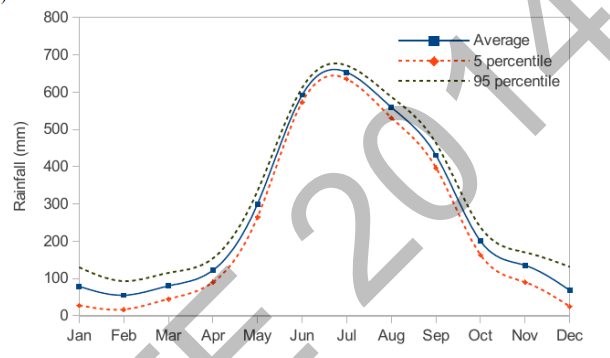
\includegraphics[width=0.7\columnwidth]{GAq10.png} \caption*{} 
        \label{fig:q10} 
    \end{figure}
    (i) On average, it rains more in July than in December \\
    (ii) Every year, the amount of rainfall in August is more than that in January \\
    (iii) July rainfall can be estimated with better confidence than February rainfall \\
    (iv) In August, there is at least $500$ mm of rainfall
    
    \hfill{\brak{\text{GATE XE 2014}}}
    \begin{enumerate}[label=\Alph*)]
        \begin{multicols}{2}
            \item (i) and (ii)
            \item (i) and (iii)
            \item (ii) and (iii)
            \item (iii) and (iv)
        \end{multicols}
    \end{enumerate}
\end{enumerate}
\clearpage

\section*{A : ENGINEERING MATHEMATICS (COMPULSORY)}
\begin{enumerate}
    \item If $1, 0$, and $-1$ are the eigenvalues of a $3\times3$ matrix A, then the trace of $A^2 + 5A$ is equal to \underline{\hspace{2cm}}.
    
    \hfill{\brak{\text{GATE XE 2014}}}

    \item Which of the following is a solution of the differential equation $x^2y''+ xy'+ y = 4\sin(\ln x), x > 0$?
    
    \hfill{\brak{\text{GATE XE 2014}}}
    \begin{enumerate}[label=\Alph*)]
        \item $y = 2x \sin(\ln x)$
        \item $y = -2x \sin(\ln x)$
        \item $y = -2\ln x \cos(\ln x)$
        \item $y = 2\ln x \cos(\ln x)$
    \end{enumerate}
    
    \item At $z=0$, the complex function $f(z)=z|z|^2$
    
    \hfill{\brak{\text{GATE XE 2014}}}
    \begin{enumerate}[label=\Alph*)]
        \item satisfies the Cauchy-Riemann equations and is differentiable
        \item satisfies the Cauchy-Riemann equations but is not differentiable.
        \item does not satisfy the Cauchy-Riemann equations but is differentiable.
        \item does not satisfy the Cauchy-Riemann equations and is not differentiable.
    \end{enumerate}
    
    \item Ten chocolates are distributed randomly among three children standing in a row. The probability that the first child receives exactly three chocolates is
    
    \hfill{\brak{\text{GATE XE 2014}}}
    \begin{enumerate}[label=\Alph*)]
        \begin{multicols}{2}
            \item $\frac{5\times2^{11}}{3^9}$
            \item $\frac{5\times2^{10}}{3^9}$
            \item $\frac{1}{3^9}$
            \item $\frac{4}{3^{10}}$
        \end{multicols}
    \end{enumerate}

    \item Let the function $f :[0,5] \rightarrow R$ be defined by
    \begin{align*}
        f(x)= 
        \begin{cases}
            2x+5, & 0\leq x<1 \\
            2x^2 +5, & 1\leq x<2 \\
            \frac{2}{3}x^3 + \frac{23}{3}, & 2\leq x\leq 5
        \end{cases}
    \end{align*}
    The number of points where $f$ is not differentiable in $(0, 5)$, is \underline{\hspace{2cm}}.
    
    \hfill{\brak{\text{GATE XE 2014}}}

    \item An integrating factor of the differential equation $(3x^2y^3e^y + y^3 + y^2) dx + (x^3y^3e^y - xy) dy = 0$ is
    
    \hfill{\brak{\text{GATE XE 2014}}}
    \begin{enumerate}[label=\Alph*)]
        \item $\frac{1}{y}$
        \item $\frac{1}{y^2}$
        \item $\frac{1}{y^3}$
        \item $\ln y$
    \end{enumerate}

    \item If a cubic polynomial passes through the points $(0, 1)$, $(1, 0)$, $(2, 1)$ and $(3, 10)$, then it also passes through the point
    
    \hfill{\brak{\text{GATE XE 2014}}}
    \begin{enumerate}[label=\Alph*)]
        \begin{multicols}{2}
            \item $(-2, -11)$
            \item $(-1, -2)$
            \item $(-1, -4)$
            \item $(-2, -23)$
        \end{multicols}
    \end{enumerate}
    
    \item Let the function $f :[0,\infty) \rightarrow R$ be such that $f'(x) = \frac{8}{x^2 + 3x + 4}$ for $x > 0$ and $f(0) = 1$. Then $f(1)$ lies in the interval
    
    \hfill{\brak{\text{GATE XE 2014}}}
    \begin{enumerate}[label=\Alph*)]
        \begin{multicols}{2}
            \item $[0, 1]$
            \item $[2, 3]$
            \item $[4, 5]$
            \item $[6, 7]$
        \end{multicols}
    \end{enumerate}

    \item The perimeter of a rectangle having the largest area that can be inscribed in the ellipse $\frac{x^2}{8} + \frac{y^2}{32} = 1$, is \underline{\hspace{2cm}}.
    
    \hfill{\brak{\text{GATE XE 2014}}}

    \item If the work done in moving a particle once around a circle $x^2 + y^2 = 4$ under the force field $\vec{F}(x,y) = (2x-ay)\hat{i} + (2y+ax)\hat{j}$ is $16\pi$, then $|a|$ is equal to \underline{\hspace{2cm}}.
    
    \hfill{\brak{\text{GATE XE 2014}}}

    \item Let $r$ and $s$ be real numbers. If $A= \myvec{1 & 2 & 0 \\ 2 & 0 & 3 \\ r & s & 0}$ and $b = \myvec{1 \\ 1 \\ s-1}$, then the system of linear equations $AX =b$ has
    
    \hfill{\brak{\text{GATE XE 2014}}}
    \begin{enumerate}[label=\Alph*)]
        \item no solutions for $s \neq 2r$.
        \item infinitely many solutions for $s = 2r \neq 2$.
        \item a unique solution for $s = 2r = 2$.
        \item infinitely many solutions for $s = 2r = 2$.
    \end{enumerate}
\end{enumerate}
\clearpage

\section*{B : FLUID MECHANICS}
\begin{enumerate}
    \item A dam with a curved shape is shown in the figure. The cross sectional area of the dam \brak{\text{shaded portion}} is $100 \text{ m}^2$ and its centroid is at $\bar{x} = 10 \text{ m}$. The vertical component of the hydrostatic force, $F_z$, is acting at a distance $x_p$. The value of $x_p$ is \underline{\hspace{2cm}} m.
    \begin{figure}[H] 
        \centering 
        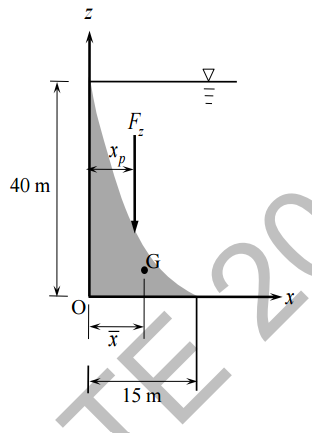
\includegraphics[width=0.4\columnwidth]{Bq1.png} \caption*{} 
        \label{fig:q1_fluid} 
    \end{figure}
    
    \hfill{\brak{\text{GATE XE 2014}}}

    \item For an unsteady incompressible fluid flow, the velocity field is $\vec{V} = (3x^2 +3)t \hat{i} - 6xyt \hat{j}$, where $x, y$ are in meters and $t$ is in seconds. Acceleration in m/s$^2$ at the point $x=10$ m and $y=0$, as measured by a stationary observer is
    
    \hfill{\brak{\text{GATE XE 2014}}}
    \begin{enumerate}[label=\Alph*)]
        \begin{multicols}{2}
            \item 303
            \item 162
            \item 43
            \item 13
        \end{multicols}
    \end{enumerate}

    \item For an incompressible flow, the existence of components of acceleration for different types of flow is described in the table below.
    \begin{table}[h!] \centering \caption*{} \label{tab:q3_fluid}
        \begin{tabular}{ll} \hline
            \textbf{Type of Flow} & \textbf{Components of Acceleration} \\ \hline
            P: Steady and uniform & 1: Local exists, convective does not exist \\
            Q: Steady and non-uniform & 2: Both exist \\
            R: Unsteady and uniform & 3: Both do not exist \\
            S: Unsteady and non-uniform & 4: Local does not exist, convective exists \\ \hline
        \end{tabular}
    \end{table}
    Which one of the following options connecting the left column with the right column is correct?
    
    \hfill{\brak{\text{GATE XE 2014}}}
    \begin{enumerate}[label=\Alph*)]
        \begin{multicols}{2}
            \item P-1; Q-4; R-3; S-2
            \item P-4; Q-1; R-2; S-3
            \item P-3; Q-2; R-1; S-4
            \item P-3; Q-4; R-1; S-2
        \end{multicols}
    \end{enumerate}

    \item Velocity in a two-dimensional flow field is specified as: $u = x^2y$; $v = -y^2x$. The magnitude of the rate of angular deformation at a location \brak{\text{$x = 2$ m and $y = 1$ m}} is \underline{\hspace{2cm}} s$^{-1}$.
    
    \hfill{\brak{\text{GATE XE 2014}}}

    \item For a plane irrotational flow, equi-potential lines and streamlines are
    
    \hfill{\brak{\text{GATE XE 2014}}}
    \begin{enumerate}[label=\Alph*)]
        \begin{multicols}{2}
            \item parallel to each other.
            \item at an angle of $90\degree$ to each other.
            \item at an angle of $45\degree$ to each other.
            \item at an angle of $60\degree$ to each other.
        \end{multicols}
    \end{enumerate}
    
    \item Flow around a Rankine half-body is represented by the superposition of
    
    \hfill{\brak{\text{GATE XE 2014}}}
    \begin{enumerate}[label=\Alph*)]
        \begin{multicols}{2}
            \item source and vortex flows.
            \item source and uniform flows.
            \item vortex and uniform flows.
            \item source, vortex and uniform flows.
        \end{multicols}
    \end{enumerate}

    \item It is required to carry out model studies on a boat having a characteristic length of $3.6$ m and travelling at a speed of $3$ m/s. Assume the acceleration due to gravity as $10$ m/s$^2$ and neglect the effects due to viscous and surface tension forces. The value of appropriate non-dimensional number is \underline{\hspace{2cm}}.
    
    \hfill{\brak{\text{GATE XE 2014}}}
    
    \item Which one of the following velocity profiles typically represents a fully developed incompressible, turbulent flow in a pipe?
    
    \hfill{\brak{\text{GATE XE 2014}}}
    \begin{figure}[H]
        \centering \caption*{} \label{fig:q8_fluid_options}
        \begin{tabular}{cccc}
        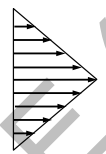
\includegraphics[width=0.2\columnwidth]{Bq8a.png} & 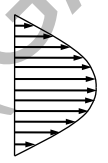
\includegraphics[width=0.2\columnwidth]{Bq8b.png} & 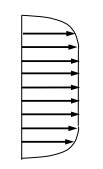
\includegraphics[width=0.2\columnwidth]{Bq8c.png} & 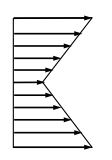
\includegraphics[width=0.2\columnwidth]{Bq8d.png} \\
        (A) & (B) & (C) & (D)
        \end{tabular}
    \end{figure}

    \item Consider an incompressible, laminar flow past a circular cylinder of diameter $d$. The flow is uniform at the far upstream. Which one of the following figures typically represents the wake velocity profile just downstream of the cylinder?
    
    \hfill{\brak{\text{GATE XE 2014}}}
    \begin{figure}[H]
        \centering \caption*{} \label{fig:q9_fluid_options}
        \begin{tabular}{cc}
        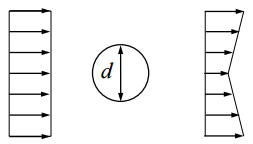
\includegraphics[width=0.3\columnwidth]{Bq9a.png} & 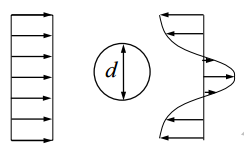
\includegraphics[width=0.3\columnwidth]{Bq9b.png} \\
        (A) & (B) \\
        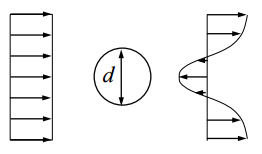
\includegraphics[width=0.3\columnwidth]{Bq9c.png} & 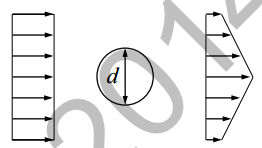
\includegraphics[width=0.3\columnwidth]{Bq9d.png} \\
        (C) & (D)
        \end{tabular}
    \end{figure}
    
    \item A container of square cross-section is partially filled with a liquid of density $\rho_1$. The cylinder is intended to float in another liquid of density $\rho_2$ as shown in the figure. The distance between metacentre and centre of buoyancy is $\frac{I_{sub}}{V_{sub}}$, where $I$ and $V_{sub}$ are area moment of inertia of the cross-section and submerged volume, respectively. Neglect the weight of the container.
    \begin{figure}[H] \centering 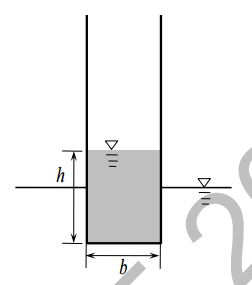
\includegraphics[width=0.3\columnwidth]{Bq10.png} \caption*{} \label{fig:q10_fluid} \end{figure}
    Which one of the following is the correct condition for stability?
    
    \hfill{\brak{\text{GATE XE 2014}}}
    \begin{enumerate}[label=\Alph*)]
        \begin{multicols}{2}
            \item $\frac{\rho_2}{\rho_1}\frac{b}{h} - \frac{h}{b}\brak{1-\frac{\rho_1}{\rho_2}} > 0$
            \item $\frac{\rho_2}{\rho_1}\frac{b}{h} - \frac{h}{b}\brak{1+\frac{\rho_1}{\rho_2}} > 0$
            \item $\frac{\rho_2}{\rho_1}\frac{b}{h} + \frac{h}{b}\brak{1-\frac{\rho_1}{\rho_2}} > 0$
            \item $\frac{\rho_2}{\rho_1}\frac{b}{h} + \frac{h}{b}\brak{1+\frac{\rho_1}{\rho_2}} > 0$
        \end{multicols}
    \end{enumerate}

    \item In a steady state two-dimensional potential flow field due to a point source, the acceleration of a particle at a distance $r$ from the point source is
    
    \hfill{\brak{\text{GATE XE 2014}}}
    \begin{enumerate}[label=\Alph*)]
        \begin{multicols}{2}
            \item proportional to $r^{-1}$.
            \item proportional to $r$.
            \item a constant.
            \item proportional to $r^{-3}$.
        \end{multicols}
    \end{enumerate}

    \item Velocity in a two-dimensional flow at time $t$ and location $(x, y)$ is described as: $\vec{V} = 3t^2 \hat{i} +(x-1)\hat{j}$. The equation for the path line of a particle passing through the point $(1,0)$ at $t=0$ is
    
    \hfill{\brak{\text{GATE XE 2014}}}
    \begin{enumerate}[label=\Alph*)]
        \begin{multicols}{2}
            \item $x^3-4y^3 = 0$
            \item $(x-1)^3 -2y^2 = 0$
            \item $(x-1)^3-64y^3 = 0$
            \item $(x+1)^4-16y^3 = 0$
        \end{multicols}
    \end{enumerate}
    
    \item The gravity driven flow over a hump of height $h$ in a canal is shown in the figure. The height of the free surface from the canal bed at upstream of the hump is $H$. The free surface height reduces to $H_1$ above the hump.
    \begin{figure}[H] \centering 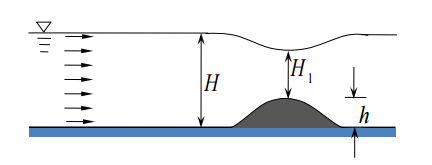
\includegraphics[width=0.6\columnwidth]{Bq13.png} \caption*{} \label{fig:q13_fluid} \end{figure}
    Assuming the canal bed to be horizontal, the discharge per unit width is given by
    
    \hfill{\brak{\text{GATE XE 2014}}}
    \begin{enumerate}[label=\Alph*)]
        \begin{multicols}{2}
            \item $\sqrt{\frac{2g(H - H_1 - h)}{\frac{1}{H_1^2} - \frac{1}{H^2}}}$
            \item $\sqrt{\frac{2gh}{\frac{1}{(H_1 + h)^2} - \frac{1}{H^2}}}$
            \item $\sqrt{\frac{2g(H - H_1)}{\frac{1}{(H_1 + h)^2} - \frac{1}{H^2}}}$
            \item $\sqrt{\frac{2g(H - H_1)}{\frac{1}{H_1^2} - \frac{1}{H^2}}}$
        \end{multicols}
    \end{enumerate}

    \item Steady state incompressible flow through a pipe network is shown in the figure. Inlets marked as (1), (2) and (3) and exit marked as (4), are shown with their respective diameters. The exit flow rate at (4) is $0.1$ m$^3$/s. A $20\%$ increase in flow rate through (3) results in a $10\%$ increase in flow rate through (4). The original velocity through inlet (3) is \underline{\hspace{2cm}} m/s.
    \begin{figure}[H] \centering 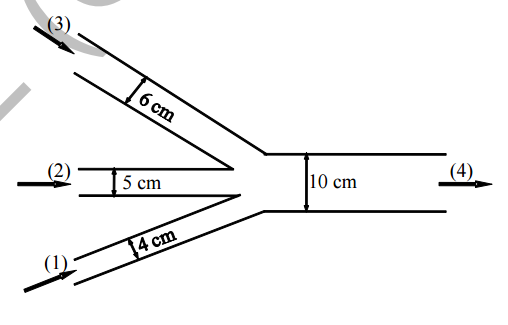
\includegraphics[width=0.6\columnwidth]{Bq14.png} \caption*{} \label{fig:q14_fluid} \end{figure}
    
    \hfill{\brak{\text{GATE XE 2014}}}

    \item A reducing elbow is used to deflect water upward by $30\degree$ as shown in the figure. The mass flow rate at the inlet is $14$ kg/s. Water is entering at a gauge pressure of $200$ kPa and exits to the atmosphere. The cross-sectional area is $113$ cm$^2$ at the inlet and $7$ cm$^2$ at the exit. Density of water and acceleration due to gravity are $1000$ kg/m$^3$ and $10$ m/s$^2$, respectively. Magnitude of $x$-component of the water force on the elbow is \underline{\hspace{2cm}} N.
    \begin{figure}[H] \centering 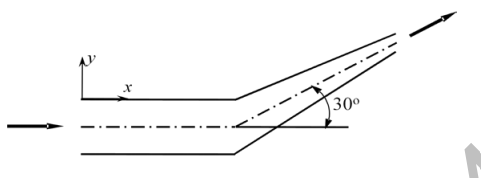
\includegraphics[width=0.6\columnwidth]{Bq15.png} \caption*{} \label{fig:q15_fluid} \end{figure}
    
    \hfill{\brak{\text{GATE XE 2014}}}

    \item A source with a strength of $k_1$ and a vortex with a strength of $k_2$ are located at the origin. The resultant velocity at a radial distance $r$ from the origin due to the superposition of the source and vortex is expressed as
    
    \hfill{\brak{\text{GATE XE 2014}}}
    \begin{enumerate}[label=\Alph*)]
        \begin{multicols}{4}
            \item $\frac{k_1 + k_2}{r}$
            \item $\frac{\sqrt{k_1^2 + k_2^2}}{r}$
            \item $\frac{\sqrt{k_2^2 - k_1^2}}{r}$
            \item $\frac{k_1 - k_2}{r}$
        \end{multicols}
    \end{enumerate}

    \item Velocity potential for an incompressible fluid flow is given as: $\phi = 2(x^2+2y-y^2)$. Assume the value of stream function at the origin to be zero. The value of stream function at $[(x,y) = (2,2)]$ is \underline{\hspace{2cm}}.
    
    \hfill{\brak{\text{GATE XE 2014}}}

    \item The model of a conduit is scaled to $1/100$ of the actual size. Seawater is used in the prototype and fresh water is used in the model. Velocity in the prototype is $0.5$ m/s. Density and dynamic viscosity of the seawater are $1025$ kg/m$^3$ and $1.07 \times 10^{-3}$ kg/m-s, respectively. Density and dynamic viscosity of fresh water are $1000$ kg/m$^3$ and $1 \times 10^{-3}$ kg/m-s, respectively. Assume the viscous forces to be dominant. The velocity to be maintained in the model to ensure dynamic similarity is \underline{\hspace{2cm}} m/s.
    
    \hfill{\brak{\text{GATE XE 2014}}}

    \item A fluid is flowing through a pipe of circular cross-section. Reynolds number of the flow is $1600$. The head loss over a $45$ m length of the pipe is $0.6$ m. The average flow velocity of the fluid is $1$ m/s and the acceleration due to gravity is $10$ m/s$^2$. The diameter of the pipe is \underline{\hspace{2cm}} m.
    
    \hfill{\brak{\text{GATE XE 2014}}}

    \item Consider a laminar flow over a flat plate of width $w$. At Section 1-1, the velocity profile is uniform as shown in the figure. The $x$-direction velocity profile at Section 2-2 is given by $\frac{u}{U} = 2\frac{y}{\delta} - \brak{\frac{y}{\delta}}^2$, where $\delta$ is the boundary layer thickness.
    \begin{figure}[H] \centering 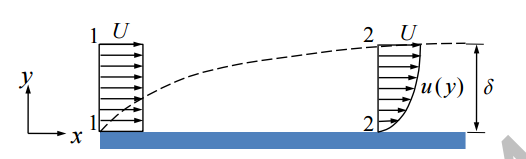
\includegraphics[width=0.7\columnwidth]{Bq20.png} \caption*{} \label{fig:q20_fluid} \end{figure}
    The volume flow rate through Section 2-2 is given by
    
    \hfill{\brak{\text{GATE XE 2014}}}
    \begin{enumerate}[label=\Alph*)]
        \begin{multicols}{4}
            \item $\frac{1}{2}U w \delta$
            \item $\frac{1}{3}U w \delta$
            \item $U w \delta$
            \item $\frac{2}{3}U w \delta$
        \end{multicols}
    \end{enumerate}
    
    \item A cube of weight $W$ and side $a$ falls at a constant speed in a medium as shown in the figure. If the medium is air \brak{\text{mass density $=\rho_{air}$}} let $U_{air}$ be the velocity of the cube. If the medium is water \brak{\text{mass density $=\rho_{water}$}} let $U_{water}$ be the velocity of the cube.
    \begin{figure}[H] \centering 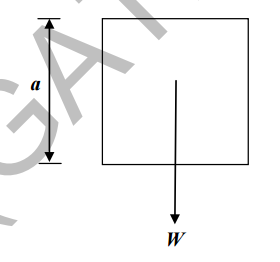
\includegraphics[width=0.3\columnwidth]{Bq21.png} \caption*{} \label{fig:q21_fluid} \end{figure}
    Neglecting the buoyancy force and assuming drag coefficient to be same for both cases, the ratio of velocities, $\brak{\frac{U_{air}}{U_{water}}}$ is given by
    
    \hfill{\brak{\text{GATE XE 2014}}}
    \begin{enumerate}[label=\Alph*)]
        \begin{multicols}{4}
            \item $\frac{\rho_{air}}{\rho_{water}}$
            \item $\sqrt{\frac{\rho_{air}}{\rho_{water}}}$
            \item $\sqrt{\frac{\rho_{water}}{\rho_{air}}}$
            \item $1$
        \end{multicols}
    \end{enumerate}

    \item Water is flowing through a venturimeter having a diameter of $0.25$ m at the entrance \brak{\text{Station 1}} and $0.125$ m at the throat \brak{\text{Station 2}} as shown in the figure. A mercury manometer measures the piezometric head difference between Stations 1 and 2 as $1.3505$ m. The loss of head between these two stations, is $1/7$ times the velocity head at the Station 2. Assume the acceleration due to gravity to be $10$ m/s$^2$. The velocity of water at the throat is \underline{\hspace{2cm}} m/s.
    \begin{figure}[H] \centering 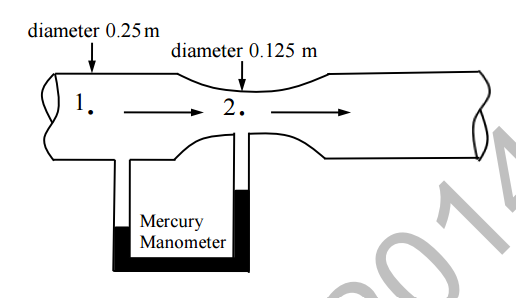
\includegraphics[width=0.6\columnwidth]{Bq22.png} \caption*{} \label{fig:q22_fluid} \end{figure}
    
    \hfill{\brak{\text{GATE XE 2014}}}
\end{enumerate}
\clearpage

\section*{C: MATERIALS SCIENCE}

Useful constants\\
Avogadro's Number: $6.023 \times 10^{23}$ mol$^{-1}$ \\
Boltzmann's constant, $k$: $1.38 \times 10^{-23}$ J.K$^{-1}$ \\
Electron Charge, $e$: $1.6 \times 10^{-19}$ C \\
Electron rest mass, $m_0$: $9.1 \times 10^{-31}$ kg \\
Universal gas constant, $R$: $8.314$ J.mol$^{-1}$.K$^{-1}$ \\
Speed of light, $c$: $3 \times 10^8$ m.s$^{-1}$ \\
Planck's constant, $h$: $6.63 \times 10^{-34}$ J.s \\
$1$ eV $= 1.6 \times 10^{-19}$ J

\begin{enumerate}
    \item Neoprene is rendered non-inflammable because
    
    \hfill{\brak{\text{GATE XE 2014}}}
    \begin{enumerate}[label=\Alph*)]
        \item it has a highly cross-linked structure
        \item it has a highly linear chain structure
        \item of the presence of chlorine atom in the structure
        \item of the absence of chlorine atom in the structure
    \end{enumerate}

    \item Nylon-6 is manufactured from
    
    \hfill{\brak{\text{GATE XE 2014}}}
    \begin{enumerate}[label=\Alph*)]
        \item caprolactum
        \item adipic acid and hexamethylene diamine
        \item maleic anhydride and hexamethylene diamine
        \item sebasic acid and hexamethylene diamine
    \end{enumerate}

    \item At room temperature, the typical barrier potential for silicon p-n junction in Volt \brak{V} is
    
    \hfill{\brak{\text{GATE XE 2014}}}
    \begin{enumerate}[label=\Alph*)]
        \begin{multicols}{4}
            \item $0.7 \times 10^{-23}$
            \item $0.07$
            \item $0.70$
            \item $7.0$
        \end{multicols}
    \end{enumerate}

    \item Quantitative measurement of the roughness of a polysilicon wafer can be performed with
    
    \hfill{\brak{\text{GATE XE 2014}}}
    \begin{enumerate}[label=\Alph*)]
        \begin{multicols}{2}
            \item scanning tunneling microscopy
            \item scanning electron microscopy
            \item transmission electron microscopy
            \item atomic force microscopy
        \end{multicols}
    \end{enumerate}

    \item The temperature of the antiferromagnetic-to-paramagnetic transition is called
    
    \hfill{\brak{\text{GATE XE 2014}}}
    \begin{enumerate}[label=\Alph*)]
        \begin{multicols}{2}
            \item Curie temperature
            \item Curie-Weiss temperature
            \item Neel temperature
            \item Debye temperature
        \end{multicols}
    \end{enumerate}

    \item At low injection level, a forward biased p-n junction would have
    
    \hfill{\brak{\text{GATE XE 2014}}}
    \begin{enumerate}[label=\Alph*)]
        \item no charge carriers
        \item minority carrier concentration much more than majority carrier concentration
        \item minority carrier concentration equal to majority carrier concentration
        \item minority carrier concentration much less than majority carrier concentration
    \end{enumerate}

    \item Which of the following mechanical properties of a material depend on the mobile dislocation density in it?
    (P) Young's modulus \quad (Q) yield strength \quad (R) ductility \quad (S) fracture toughness
    
    \hfill{\brak{\text{GATE XE 2014}}}
    \begin{enumerate}[label=\Alph*)]
        \begin{multicols}{4}
            \item P, Q, R
            \item Q, R, S
            \item P, R, S
            \item S, P, Q
        \end{multicols}
    \end{enumerate}

    \item The equilibrium concentration of vacancies in a pure metal
    
    \hfill{\brak{\text{GATE XE 2014}}}
    \begin{enumerate}[label=\Alph*)]
        \item increases exponentially with temperature
        \item decreases exponentially with temperature
        \item varies linearly with temperature
        \item is independent of temperature
    \end{enumerate}
    
    \item The materials belonging to which one of the following crystal classes would be both piezoelectric and ferroelectric
    
    \hfill{\brak{\text{GATE XE 2014}}}
    \begin{enumerate}[label=\Alph*)]
        \begin{multicols}{4}
            \item 222
            \item 4mm
            \item $\bar{1}$
            \item 2/m
        \end{multicols}
    \end{enumerate}
    
    \item Polymerized isotactic polybutadiene has a molecular weight of $3 \times 10^5$ g/mol. The degree of polymerization is \underline{\hspace{2cm}}.
    
    \hfill{\brak{\text{GATE XE 2014}}}
    
    \item A bar of Ti with Young's modulus of $110$ GPa and yield strength of $880$ MPa is tested in tension. It is noticed that the alloy does not exhibit any strain hardening and fails at a total strain of $0.108$. The mechanical energy that is necessary to break the material in MJ/m$^3$ is \underline{\hspace{2cm}}.
    
    \hfill{\brak{\text{GATE XE 2014}}}
    
    \item A copper cup weighing $140$ g contains $80$ g of water at $4 \degree$C. Specific heats of water and copper are $4.18$ and $0.385$ J/g $\degree$C, respectively. If $100$ g of water that is at $90 \degree$C is added to the cup, the final temperature of water in $\degree$C is \underline{\hspace{2cm}}.
    
    \hfill{\brak{\text{GATE XE 2014}}}
    
    \item Match the reaction in Column I with its name in Column II.
    $L$ - liquid, $\alpha, \beta, \gamma$ - different solid solution phases
    \begin{table}[h!] \centering \caption*{} \label{tab:q13_material}
        \begin{tabular}{|l|l|} \hline
            \textbf{Column I} & \textbf{Column II} \\ \hline
            (P) $L \xrightarrow{\text{cooling}} \alpha + \beta$ & (1) peritectic \\
            (Q) $L + \beta \xrightarrow{\text{cooling}} \gamma$ & (2) eutectic \\
            (R) $\alpha \xrightarrow{\text{cooling}} \beta + \gamma$ & (3) monotectic \\
            & (4) eutectoid \\ \hline
        \end{tabular}
    \end{table}
    
    \hfill{\brak{\text{GATE XE 2014}}}
    \begin{enumerate}[label=\Alph*)]
        \begin{multicols}{2}
            \item P-1, Q-4, R-3
            \item P-2, Q-1, R-4
            \item P-2, Q-3, R-1
            \item P-4, Q-2, R-3
        \end{multicols}
    \end{enumerate}

    \item The Young's modulus of a unidirectional SiC fiber reinforced Ti matrix composite is $185$ GPa. If the Young's moduli of Ti and SiC are $110$ and $360$ GPa respectively, the volume fraction of fibers in the composite is \underline{\hspace{2cm}}.
    
    \hfill{\brak{\text{GATE XE 2014}}}

    \item Match the composite in Column I with the most suitable application in Column II.
    \begin{table}[h!] \centering \caption*{} \label{tab:q15_material}
        \begin{tabular}{ll} \hline
            \textbf{Column I} & \textbf{Column II} \\ \hline
            (P) Glass fibre reinforced plastic & (1) Missile cone heads \\
            (Q) SiC particle reinforced Al alloy & (2) Commercial automobile chasis \\
            (R) Carbon-carbon composite & (3) Airplane wheel tyres \\
            (S) Metal fibre reinforced rubber & (4) Car piston rings \\
            & (5) High performance skate boards \\ \hline
        \end{tabular}
    \end{table}
    
    \hfill{\brak{\text{GATE XE 2014}}}
    \begin{enumerate}[label=\Alph*)]
        \begin{multicols}{2}
            \item P-4, Q-5, R-1, S-2
            \item P-3, Q-5, R-2, S-4
            \item P-5, Q-4, R-1, S-3
            \item P-4, Q-2, R-3, S-1
        \end{multicols}
    \end{enumerate}
    
    \item Which among the following rules need to be satisfied for obtaining an isomorphous phase diagram in a binary alloy system?
    (P) The atomic size difference should be less than $15\%$. \\
    (Q) Both the end components should have the same crystal structure \\
    (R) The valency of the end components should be the same. \\
    (S) The end components should have dissimilar electronegativities
    
    \hfill{\brak{\text{GATE XE 2014}}}
    \begin{enumerate}[label=\Alph*)]
        \begin{multicols}{4}
            \item P, Q, R
            \item Q, R, S
            \item R, S, P
            \item S, P, Q
        \end{multicols}
    \end{enumerate}
    
    \item The energy in eV and the wavelength in $\mu$m, respectively, of the photon emitted when an electron in a hydrogen atom falls from $n = 4$ to $n = 2$ state is
    
    \hfill{\brak{\text{GATE XE 2014}}}
    \begin{enumerate}[label=\Alph*)]
        \begin{multicols}{4}
            \item $3.0$, $0.413$
            \item $2.55$, $0.365$
            \item $2.75$, $0.451$
            \item $2.55$, $0.487$
        \end{multicols}
    \end{enumerate}
    
    \item The weight in kg of gallium \brak{Ga} to be mixed with arsenic \brak{\text{As}} for obtaining $1.0$ kg of gallium arsenide \brak{\text{GaAs}} is \underline{\hspace{2cm}}. \brak{\text{$M_{Ga} = 69.72$ g/mol, $M_{As} = 74.92$ g/mol}}
    
    \hfill{\brak{\text{GATE XE 2014}}}

    \item Match the material in Column I with the property in Column II
    \begin{table}[h!] \centering \caption*{} \label{tab:q19_material}
        \begin{tabular}{ll} \hline
            \textbf{Column I} & \textbf{Column II} \\ \hline
            (P) Pb(Zr,Ti)O$_3$ & (1) Shape memory alloy \\
            (Q) Ni$_{50}$Ti$_{50}$ & (2) Piezoelectric ceramic \\
            (R) GaAs & (3) High temperature superconductor \\
            (S) YBa$_2$Cu$_3$O$_7$ & (4) Optoelectronic semiconductor \\ \hline
        \end{tabular}
    \end{table}
    
    \hfill{\brak{\text{GATE XE 2014}}}
    \begin{enumerate}[label=\Alph*)]
        \begin{multicols}{2}
            \item P-1, Q-2, R-3, S-4
            \item P-2, Q-3, R-4, S-1
            \item P-4, Q-1, R-2, S-3
            \item P-2, Q-1, R-4, S-3
        \end{multicols}
    \end{enumerate}

    \item Relevant portion of a binary phase diagram of elements A and B is shown below. The mass fraction of liquid phase at $1000 \degree$C for an alloy with $15$ wt.\% B is \underline{\hspace{2cm}}.
    \begin{figure}[H] \centering 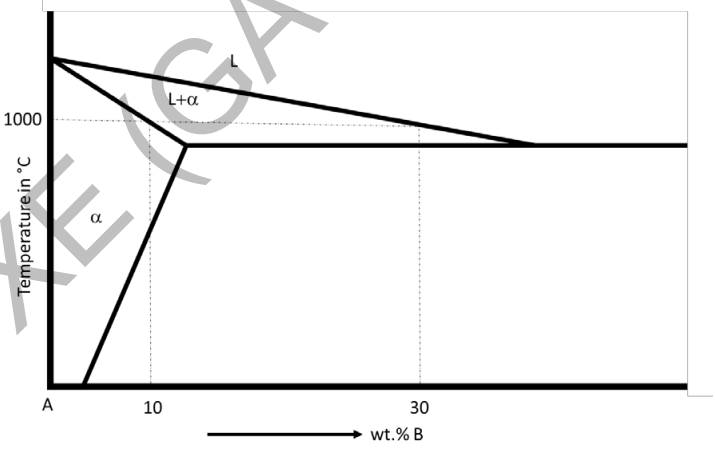
\includegraphics[width=0.6\columnwidth]{q20_material.png} \caption*{} \label{fig:q20_material} \end{figure}
    
    \hfill{\brak{\text{GATE XE 2014}}}

    \item The expected diffraction angle (in degrees) for the first order reflection from the (113) set of planes for face centered cubic Pt (lattice parameter = $0.392$ nm) using monochromatic radiation of wavelength $0.1542$ nm is \underline{\hspace{2cm}}.
    
    \hfill{\brak{\text{GATE XE 2014}}}
    
    \item The diffusion coefficients of Mg in Al at $500$ and $550 \degree$C are $1.9 \times 10^{-13}$ and $5.8 \times 10^{-13}$ m$^2$/s respectively. The activation energy for diffusion of Mg in Al in kJ/mol is \underline{\hspace{2cm}}.
    
    \hfill{\brak{\text{GATE XE 2014}}}
\end{enumerate}
\clearpage

\section*{D: SOLID MECHANICS}
\begin{enumerate}
    \item A steel wire of diameter $5$ mm is bent around a cylindrical drum of radius $0.5$ m. The steel wire has modulus of elasticity of $200$ GPa. Find the bending moment in the wire in N-m.
    \begin{figure}[H] \centering 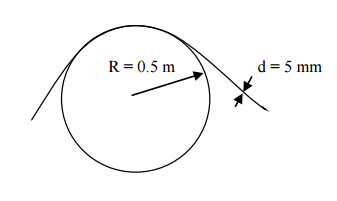
\includegraphics[width=0.4\columnwidth]{q1_solid.png} \caption*{} \label{fig:q1_solid} \end{figure}
    
    \hfill{\brak{\text{GATE XE 2014}}}

    \item A compressed air tank having an inner diameter of $480$ mm and a wall thickness of $8$ mm is formed by welding two steel hemispheres. If the allowable shear stress in the steel is $40$ MPa, find the maximum permissible pressure (in MPa) inside the tank.
    
    \hfill{\brak{\text{GATE XE 2014}}}

    \item The Euler's buckling load of a column fixed at both the ends is $P$. If one of the ends is made free, the buckling load shall change to
    
    \hfill{\brak{\text{GATE XE 2014}}}
    \begin{enumerate}[label=\Alph*)]
        \begin{multicols}{2}
            \item $P/16$
            \item $P/8$
            \item $P/4$
            \item $P/2$
        \end{multicols}
    \end{enumerate}

    \item A point in a body is subjected to a bi-axial state of stress, equal in magnitude but opposite in nature. On a plane inclined at an angle $45\degree$ with respect to x-axis (passing through the point), the
    
    \hfill{\brak{\text{GATE XE 2014}}}
    \begin{enumerate}[label=\Alph*)]
        \item shear and normal stresses are zero
        \item normal stress is maximum and shear stress is zero
        \item shear stress is maximum and normal stress is zero
        \item shear stress is maximum and normal stress is non-zero
    \end{enumerate}

    \item A weightless beam subjected to two point loads is shown in the figure below.
    \begin{figure}[H] \centering 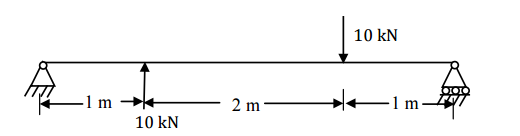
\includegraphics[width=0.6\columnwidth]{q5_solid.png} \caption*{} \label{fig:q5_solid} \end{figure}
    The shear force diagram of the beam is
    
    \hfill{\brak{\text{GATE XE 2014}}}
    \begin{figure}[H] \centering \caption*{} \label{fig:q5_solid_options}
        (A) 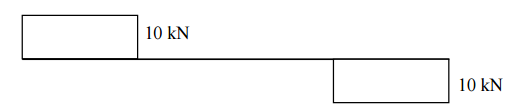
\includegraphics[width=0.5\columnwidth]{q5a_solid.png} \\
        (B) 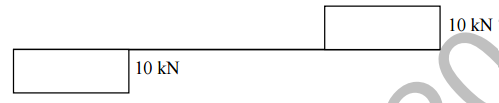
\includegraphics[width=0.5\columnwidth]{q5b_solid.png} \\
        (C) 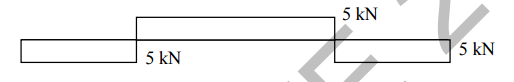
\includegraphics[width=0.5\columnwidth]{q5c_solid.png} \\
        (D) 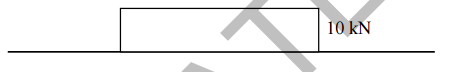
\includegraphics[width=0.5\columnwidth]{q5d_solid.png}
    \end{figure}
    
    \item For the pin jointed truss, find the axial force (in kN) in the member 2-5.
    \begin{figure}[H] \centering 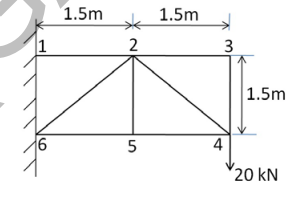
\includegraphics[width=0.4\columnwidth]{q6_solid.png} \caption*{} \label{fig:q6_solid} \end{figure}
    
    \hfill{\brak{\text{GATE XE 2014}}}

    \item The supporting structure of a water tank is made of reinforced concrete (RC) with a tubular cross section of inner diameter $d_i$, outer diameter $d_o$, height $l$, and Young's modulus $E$. The mass of the tank is $m$. If mass of the supporting structure is neglected, then the natural frequency of the water tank in transverse direction is
    
    \hfill{\brak{\text{GATE XE 2014}}}
    \begin{enumerate}[label=\Alph*)]
        \begin{multicols}{2}
            \item $\sqrt{\frac{3\pi E(d_o^4 - d_i^4)}{64l^3m}}$
            \item $\sqrt{\frac{\pi E(d_o^4 - d_i^4)}{8l^3m}}$
            \item $\sqrt{\frac{384\pi E(d_o^4 - d_i^4)}{360l^3m}}$
            \item $\sqrt{\frac{\pi E(d_o^4 - d_i^4)}{64l^3m}}$
        \end{multicols}
    \end{enumerate}

    \item A mass is attached to a spring and placed horizontally in a frictionless surface. A simple pendulum has been pivoted to the mass. The degree of freedom of this system is
    \begin{figure}[H] \centering 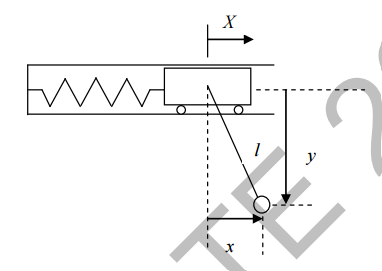
\includegraphics[width=0.5\columnwidth]{q8_solid.png} \caption*{} \label{fig:q8_solid} \end{figure}
    
    \hfill{\brak{\text{GATE XE 2014}}}
    \begin{enumerate}[label=\Alph*)]
        \begin{multicols}{4}
            \item 1
            \item 2
            \item 3
            \item 4
        \end{multicols}
    \end{enumerate}

    \item Consider the following two statements
    Statement 1: A body of weight $W$ falls from a height $h$ and strikes the ground. If the body starts from rest, the velocity with which it strikes the ground is $\sqrt{2gh}$, where $g$ is the acceleration due to gravity.
    \begin{figure}[H] \centering 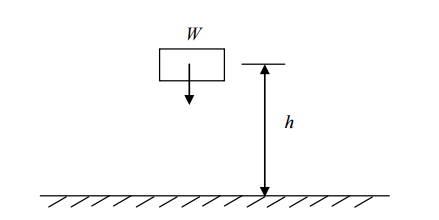
\includegraphics[width=0.3\columnwidth]{q9_solid_1.png} \caption*{} \label{fig:q9_solid_1} \end{figure}
    Statement 2: If the same body (initially at rest) slides without friction along an inclined plane $PQ$ (angle of inclination $\alpha$) starting from an elevation $h$ above point $Q$, then its velocity at point $Q$ is $\sqrt{2gh}$.
    \begin{figure}[H] \centering 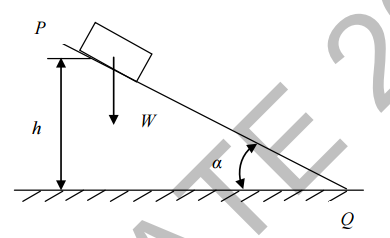
\includegraphics[width=0.4\columnwidth]{q9_solid_2.png} \caption*{} \label{fig:q9_solid_2} \end{figure}
    The correct option is
    
    \hfill{\brak{\text{GATE XE 2014}}}
    \begin{enumerate}[label=\Alph*)]
        \item Both statements 1 and 2 are true
        \item Statement 1 is true and 2 is false
        \item Statement 1 is false and 2 is true
        \item Both statements 1 and 2 are false
    \end{enumerate}

    \item A composite bar of length 'L' is made of a centrally placed steel plate (50 mm wide x 10 mm thick) with two copper plates (each 30 mm wide x 5 mm thick) connected rigidly on each side. If the temperature of the composite bar is raised by $50 \degree$C, find the stress developed in each copper plate in MPa.
    (For Steel: $E_s = 2 \times 10^5$ MPa and $\alpha_s = 12 \times 10^{-6} / \degree$C; For Copper: $E_c = 1 \times 10^5$ MPa and $\alpha_c = 17 \times 10^{-6} / \degree$C)
    \begin{figure}[H] \centering 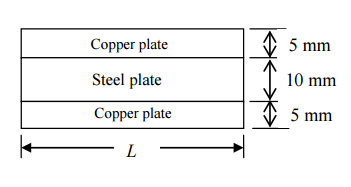
\includegraphics[width=0.5\columnwidth]{q10_solid.png} \caption*{} \label{fig:q10_solid} \end{figure}
    
    \hfill{\brak{\text{GATE XE 2014}}}

    \item The vertical deflection at the free end of the cantilever beam as shown in figure is
    \begin{figure}[H] \centering 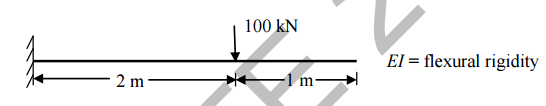
\includegraphics[width=0.5\columnwidth]{q11_solid.png} \caption*{} \label{fig:q11_solid} \end{figure}
    
    \hfill{\brak{\text{GATE XE 2014}}}
    \begin{enumerate}[label=\Alph*)]
        \begin{multicols}{2}
            \item $1400/EI$
            \item $1400/3EI$
            \item $200/EI$
            \item $100/EI$
        \end{multicols}
    \end{enumerate}
    
    \item A hollow shaft and a solid shaft have the same length and the same outer radius $R$. The inner radius of the hollow shaft is $0.6 R$. Assuming that both the shafts are made of same material and are subjected to the same torque, find the ratio of shear stress in hollow shaft to that in solid shaft.
    
    \hfill{\brak{\text{GATE XE 2014}}}
    
    \item A beam with overhangs carries one point load acting downwards and the other upward. The clockwise moment $Pb$ is applied at each support. The bending moment at the midpoint of the beam is
    \begin{figure}[H] \centering 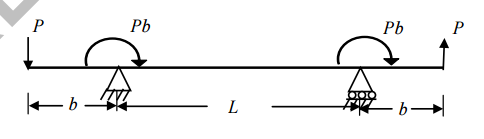
\includegraphics[width=0.7\columnwidth]{q13_solid.png} \caption*{} \label{fig:q13_solid} \end{figure}
    
    \hfill{\brak{\text{GATE XE 2014}}}
    \begin{enumerate}[label=\Alph*)]
        \begin{multicols}{4}
            \item 0
            \item $PL/2$
            \item $PL$
            \item $PbL$
        \end{multicols}
    \end{enumerate}
    
    \item A cantilever beam of length $L$ supports a concentrated load $P$ at the free end. The cross section of the beam is rectangular with constant width $b$ and varying depth $h$. The depth $h$ of this idealized cantilever beam varies in such a way that the maximum normal stress at every cross section remains equal to the allowable bending stress. Considering only the bending stresses, the depth $h_x$ of the fully stressed beam at any distance $x$ from the free end shall vary
    \begin{figure}[H] \centering 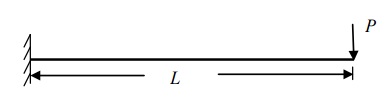
\includegraphics[width=0.6\columnwidth]{q14_solid.png} \caption*{} \label{fig:q14_solid} \end{figure}
    
    \hfill{\brak{\text{GATE XE 2014}}}
    \begin{enumerate}[label=\Alph*)]
        \begin{multicols}{2}
            \item with square of $x$
            \item with square root of $x$
            \item linearly with $x$
            \item with cube of $x$
        \end{multicols}
    \end{enumerate}
    
    \item A cantilever beam is subjected to following three different loading conditions:
    (a) a concentrated load $P$ at its free end,
    (b) a couple $M_o$ at its free end and
    (c) both loads acting simultaneously
    \begin{figure}[H] \centering 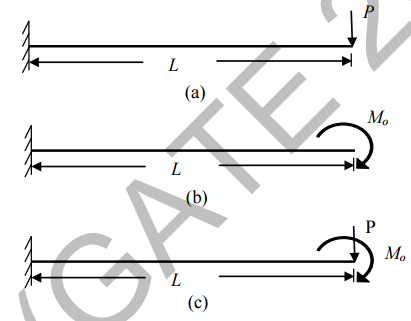
\includegraphics[width=0.4\columnwidth]{q15_solid.png} \caption*{} \label{fig:q15_solid} \end{figure}
    The flexural rigidity of the beam may be assumed as $EI$. The strain energy due to bending when both loads act simultaneously
    
    \hfill{\brak{\text{GATE XE 2014}}}
    \begin{enumerate}[label=\Alph*)]
        \item can be determined by applying the principle of superposition and the strain energy is $\frac{P^2L^3}{6EI} + \frac{M_o^2 L}{2EI}$
        \item can be determined by applying the principle of superposition and the strain energy is $\frac{P^2L^2}{6EI} + \frac{M_o L^3}{2EI}$
        \item cannot be determined by applying the principle of superposition and the strain energy is $\frac{P^2L^3}{6EI} + \frac{M_o^2 L}{2EI} + \frac{P M_o L^2}{2EI}$
        \item cannot be determined by applying the principle of superposition and the strain energy is $\frac{P^2L^2}{6EI} + \frac{M_o L^3}{2EI} + \frac{P M_o L^2}{2EI}$
    \end{enumerate}
    
    \item A tapered rod has diameter $d_1$ at one end which reduces uniformly to a diameter $d_2$ over the length ($L$). If the modulus of elasticity of the material is $E$, the change in the length of the rod due to the application of axial force ($P$) is
    
    \hfill{\brak{\text{GATE XE 2014}}}
    \begin{enumerate}[label=\Alph*)]
        \begin{multicols}{2}
            \item $\frac{4PL}{\pi E d_1 d_2}$
            \item $\frac{4PL}{\pi E (d_1^2 - d_2^2)}$
            \item $\frac{PL}{\pi E d_1 d_2}$
            \item $\frac{2PL}{\pi E (d_1^2 - d_2^2)}$
        \end{multicols}
    \end{enumerate}
    
    \item For a point in a body subjected to a plane stress condition ($\sigma_x = 100$ MPa, $\sigma_y = 50$ MPa and $\tau_{xy} = \tau_{yx} = 25$ MPa), the maximum principal stress in MPa is \underline{\hspace{2cm}}.
    
    \hfill{\brak{\text{GATE XE 2014}}}
    
    \item An isotropic body is subjected to a state of stress given by: $\sigma_x = 10$ MPa and $\tau_{xy} = \tau_{yx} = -20$ MPa. Assuming $G=0.4E$, the volumetric strain is
    
    \hfill{\brak{\text{GATE XE 2014}}}
    \begin{enumerate}[label=\Alph*)]
        \begin{multicols}{4}
            \item 5/E
            \item 7.5/E
            \item 10/E
            \item 15/E
        \end{multicols}
    \end{enumerate}
    
    \item A block of weight $Q$ rests on an inclined plane and it is attached to a string which runs over a frictionless pulley to carry a block of weight $P$ at its other end. The coefficient of friction between the block of weight $Q$ and the inclined plane is $\mu$. Consider the following cases:
    Case I: weight $Q$ starts moving down the inclined plane
    Case II: weight $P$ starts falling down
    \begin{figure}[H] \centering 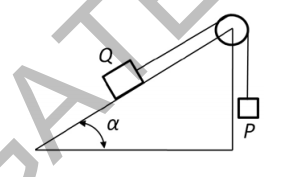
\includegraphics[width=0.4\columnwidth]{q19_solid.png} \caption*{} \label{fig:q19_solid} \end{figure}
    The limiting values of ratio $P/Q$ for Case I and Case II respectively are
    
    \hfill{\brak{\text{GATE XE 2014}}}
    \begin{enumerate}[label=\Alph*)]
        \item $(\sin\alpha - \mu\cos\alpha)$ and $(\sin\alpha + \mu\cos\alpha)$
        \item $(\mu\sin\alpha - \cos\alpha)$ and $(\mu\sin\alpha + \cos\alpha)$
        \item $(\sin\alpha + \mu\cos\alpha)$ and $(\sin\alpha - \mu\cos\alpha)$
        \item $(\mu\sin\alpha + \cos\alpha)$ and $\mu(\sin\alpha - \cos\alpha)$
    \end{enumerate}
    
    \item To unload an item from a truck a crane boom is raised with a constant angular velocity of $1$ rad/s relative to the cab and then the cab is rotated about a vertical axis with constant angular velocity of $0.5$ rad/s.
    \begin{figure}[H] \centering 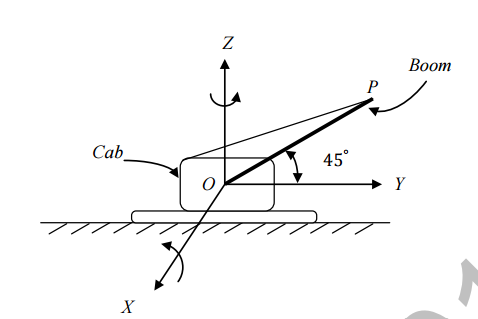
\includegraphics[width=0.6\columnwidth]{q20_solid.png} \caption*{} \label{fig:q20_solid} \end{figure}
    If the length of the boom ($OP$) is $10$ m, the velocity of the tip ($P$) of the boom in m/s is
    
    \hfill{\brak{\text{GATE XE 2014}}}
    \begin{enumerate}[label=\Alph*)]
        \begin{multicols}{2}
            \item $\frac{5}{\sqrt{2}}(-2\hat{i} - \hat{j} + 2\hat{k})$
            \item $\frac{5}{\sqrt{2}}(-\hat{i} - 2\hat{j} + \hat{k})$
            \item $\frac{5}{\sqrt{2}}(-2\hat{i} - \hat{j} + 2\hat{k})$
            \item $\frac{5}{\sqrt{2}}(-\hat{i} - 2\hat{j} + 2\hat{k})$
        \end{multicols}
    \end{enumerate}

    \item A block of mass $5$ kg moves up on a smooth inclined plane with a velocity of $10$ m/s in the direction shown. A bullet of mass $60$ g travelling at $500$ m/s strikes the block centrally and gets embedded in it. The velocity of the block and embedded bullet in m/s immediately after the impact is
    \begin{figure}[H] \centering 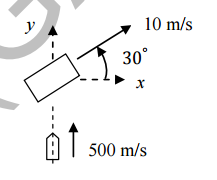
\includegraphics[width=0.4\columnwidth]{q21_solid.png} \caption*{} \label{fig:q21_solid} \end{figure}
    
    \hfill{\brak{\text{GATE XE 2014}}}
    \begin{enumerate}[label=\Alph*)]
        \begin{multicols}{4}
            \item 12.54 at $30\degree$
            \item 13.84 at $51.78\degree$
            \item 13.84 at $30\degree$
            \item 15.62 at $51.78\degree$
        \end{multicols}
    \end{enumerate}
    
    \item A balloon with ballast (weight) inside it has a gross weight of $500$ N. It is falling vertically with a constant acceleration of $2$ m/s$^2$. If air resistance is negligible, find the weight of ballast (in N) that must be thrown out in order to give the balloon an upward acceleration of $2$ m/s$^2$. (Acceleration due to gravity, $g = 9.81$ m/s$^2$)
    \begin{figure}[H] \centering 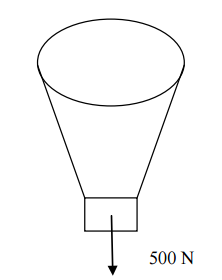
\includegraphics[width=0.3\columnwidth]{q22_solid.png} \caption*{} \label{fig:q22_solid} \end{figure}
    
    \hfill{\brak{\text{GATE XE 2014}}}
\end{enumerate}
\clearpage

\section*{E: THERMODYNAMICS}
Notations used: \\
$P$-pressure, $V$-volume, $T$-temperature, $S$-entropy, $H$-enthalpy, $U$-internal energy, $c_p$-specific heat at constant pressure, $c_v$-specific heat at constant volume; specific properties are designated by lower case symbols.
Subscripts: R-reduced, C-critical, f-saturated liquid, g-saturated vapor. \\
Properties of air: $c_p = 1.005$ kJ/(kg.K), specific heat ratio $\gamma = 1.4$, Gas constant $= 0.287$ kJ/(kg.K), Molecular weight $= 29$ gm/mol. \\
Universal gas constant $= 8.314$ kJ/(kmol.K).

\begin{enumerate}
    \item Entropy is a
    
    \hfill{\brak{\text{GATE XE 2014}}}
    \begin{enumerate}[label=\Alph*)]
        \begin{multicols}{2}
            \item Path function
            \item Point function
            \item Property independent function
            \item Neither path nor point function
        \end{multicols}
    \end{enumerate}

    \item A small container has gas at high pressure. It is placed in an evacuated space. If the container is punctured, work done by the gas is
    
    \hfill{\brak{\text{GATE XE 2014}}}
    \begin{enumerate}[label=\Alph*)]
        \begin{multicols}{4}
            \item Positive
            \item Negative
            \item Zero
            \item $\infty$
        \end{multicols}
    \end{enumerate}

    \item The molecular weight of a mixture is $38.4$ gm/mol. The mixture is composed of methane and carbon-dioxide gases. The atomic weights of the elements C, H, and O are $12, 1$, and $16$ gm/mol, respectively. The mole fraction of methane ($X_{methane}$) is \underline{\hspace{2cm}} and that of carbon-dioxide ($X_{carbon-dioxide}$) is \underline{\hspace{2cm}}.
    
    \hfill{\brak{\text{GATE XE 2014}}}
    \begin{enumerate}[label=\Alph*)]
        \item $X_{methane} = 0.2; X_{carbon-dioxide} = 0.8$
        \item $X_{methane} = 0.8; X_{carbon-dioxide} = 0.2$
        \item $X_{methane} = 0.3; X_{carbon-dioxide} = 0.7$
        \item $X_{methane} = 0.7; X_{carbon-dioxide} = 0.3$
    \end{enumerate}

    \item A system undergoes a change from state 1 to state 2. During this process, the change in the internal energy is $\Delta U$. The change in internal energy of the system when executing the cycle 1-2-1 is equal to
    
    \hfill{\brak{\text{GATE XE 2014}}}
    \begin{enumerate}[label=\Alph*)]
        \begin{multicols}{4}
            \item $\Delta U$
            \item $2\Delta U$
            \item Zero
            \item $-2\Delta U$
        \end{multicols}
    \end{enumerate}

    \item Which among the following plots represents a line joining two states with the same dew point temperature on a standard psychrometric chart, with the dry bulb temperature on the X-axis and the humidity ratio on the Y-axis?
    
    \hfill{\brak{\text{GATE XE 2014}}}
    \begin{figure}[H]
        \centering \caption*{} \label{fig:q5_thermo_options}
        \begin{tabular}{cc}
        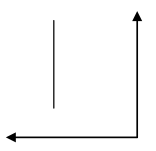
\includegraphics[width=0.3\columnwidth]{   q5a_thermo.png} & 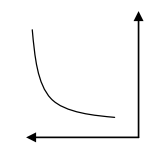
\includegraphics[width=0.3\columnwidth]{q5b_thermo.png} \\
        (A) & (B) \\
        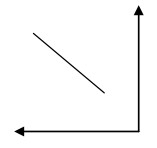
\includegraphics[width=0.3\columnwidth]{q5c_thermo.png} & 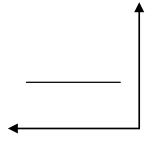
\includegraphics[width=0.3\columnwidth]{q5d_thermo.png} \\
        (C) & (D)
        \end{tabular}
    \end{figure}
    
    \item The efficiency of a reversible engine operating between two temperatures is $40\%$. The COP of a reversible refrigerator operating between the same temperatures is
    
    \hfill{\brak{\text{GATE XE 2014}}}
    \begin{enumerate}[label=\Alph*)]
        \begin{multicols}{4}
            \item 1.5
            \item 2.5
            \item 0.4
            \item 3.5
        \end{multicols}
    \end{enumerate}
    
    \item For a superheated vapor that cannot be approximated as an ideal gas, the expression determining a small change in the specific internal energy is
    
    \hfill{\brak{\text{GATE XE 2014}}}
    \begin{enumerate}[label=\Alph*)]
        \item $du = c_p dT + \brak{\frac{\partial u}{\partial v}}_T dv$
        \item $du = c_v dT + \brak{\frac{\partial u}{\partial P}}_T dP$
        \item $du = c_v dT + \brak{\frac{\partial u}{\partial v}}_T dv$
        \item $du = c_v dT$
    \end{enumerate}
    
    \item The minimum and maximum volumes in an air standard Otto cycle are $100$ and $800$ cm$^3$. Its thermal efficiency (\%) is
    
    \hfill{\brak{\text{GATE XE 2014}}}
    \begin{enumerate}[label=\Alph*)]
        \begin{multicols}{4}
            \item 56.47
            \item 94.55
            \item 54.08
            \item 87.50
        \end{multicols}
    \end{enumerate}

    \item At a saturation temperature $T_{sat}$, the difference between the entropy of saturated vapor and entropy of saturated liquid can be expressed as
    
    \hfill{\brak{\text{GATE XE 2014}}}
    \begin{enumerate}[label=\Alph*)]
        \begin{multicols}{2}
            \item $(h_f - h_g) / T_{sat}$
            \item $(h_g - h_f) / T_{sat}$
            \item $(u_g - u_f) / T_{sat}$
            \item $(u_f - u_g) / T_{sat}$
        \end{multicols}
    \end{enumerate}

    \item A gas in a closed system is compressed reversibly from an initial volume of $0.2$ m$^3$ to $0.1$ m$^3$ at a constant pressure of $3$ bar. During this process, there was a heat transfer of $50$ kJ from the gas. The change in internal energy of the gas during this process in kJ is
    
    \hfill{\brak{\text{GATE XE 2014}}}
    \begin{enumerate}[label=\Alph*)]
        \begin{multicols}{4}
            \item 20
            \item -80
            \item 80
            \item -20
        \end{multicols}
    \end{enumerate}

    \item In a closed rigid vessel, air is initially at a pressure of $0.3$ MPa and volume of $0.1$ m$^3$ at $300$ K. A stirrer supplies $100$ kJ of work to the air, while $20$ kJ of heat is lost to the atmosphere across the container walls. After these processes, the temperature of air changes to \underline{\hspace{2cm}} K.
    \begin{figure}[H] \centering 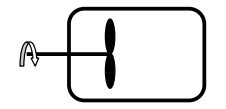
\includegraphics[width=0.4\columnwidth]{q11_thermo.png} \caption*{} \label{fig:q11_thermo} \end{figure}
    
    \hfill{\brak{\text{GATE XE 2014}}}
    \begin{enumerate}[label=\Alph*)]
        \begin{multicols}{4}
            \item 321.9
            \item 702.4
            \item 782.4
            \item 620.2
        \end{multicols}
    \end{enumerate}

    \item A reversible heat engine (E) operates using three thermal reservoirs with temperatures as shown in the following figure. If $Q_1 = Q_2$, the efficiency of the engine is \underline{\hspace{2cm}}.
    \begin{figure}[H] \centering 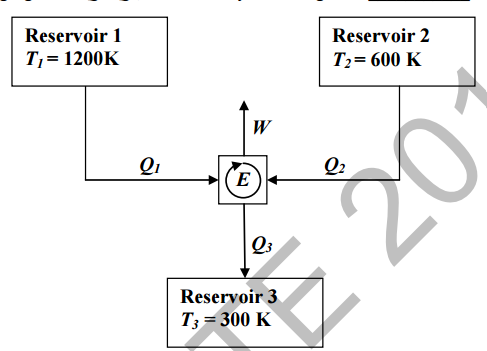
\includegraphics[width=0.6\columnwidth]{q12_thermo.png} \caption*{} \label{fig:q12_thermo} \end{figure}
    
    \hfill{\brak{\text{GATE XE 2014}}}
    \begin{enumerate}[label=\Alph*)]
        \begin{multicols}{4}
            \item 0.25
            \item 0.125
            \item 0.625
            \item 0.75
        \end{multicols}
    \end{enumerate}
    
    \item A metal block of mass $25$ kg at $300$ K is immersed in an infinitely large liquid nitrogen bath maintained at $77$ K. The system comprising of the block and liquid nitrogen attains thermal equilibrium. The average specific heat of the metal is $0.45$ kJ/(kg.K). The entropy generated during the process is \underline{\hspace{2cm}} kJ/K.
    
    \hfill{\brak{\text{GATE XE 2014}}}
    \begin{enumerate}[label=\Alph*)]
        \begin{multicols}{4}
            \item 17.28
            \item 32.5
            \item 47.8
            \item -47.8
        \end{multicols}
    \end{enumerate}

    \item For a gas obeying the equation of state given by $\brak{P + \frac{a}{v^2}}v = RT$, the values of the critical volume and the critical temperature are $0.004$ m$^3$/kg and $100 \degree$C, respectively. If the value of the gas constant is $250$ J/(kg.K), then the value of the constant '$a$' is \underline{\hspace{2cm}} (N.m$^4$/kg$^2$). Note that the critical point is the point of inflection on the critical isotherm.
    
    \hfill{\brak{\text{GATE XE 2014}}}
    \begin{enumerate}[label=\Alph*)]
        \begin{multicols}{4}
            \item 124.3
            \item 0.75
            \item 186.58
            \item 248.67
        \end{multicols}
    \end{enumerate}

    \item A rigid closed vessel is initially filled with $2$ kg of water which is a mixture of saturated liquid and saturated vapor states at $2$ bar. The vessel is placed in an oven which heats the mixture to the critical state. Using the saturated and critical property values from the table given below, the heat transferred from the oven to the vessel is \underline{\hspace{2cm}} kJ.
    \begin{table}[h!] \centering \caption*{} \label{tab:q15_thermo}
        \begin{tabular}{|l|c|c|c|c|} \hline
            \multicolumn{5}{|c|}{Pressure = 2 bar} \\ \hline
            & $v_f$(m$^3$/kg) & $v_g$(m$^3$/kg) & $u_f$(kJ/kg) & $u_g$(kJ/kg) \\ \hline
            & 0.0010605 & 0.8857 & 504.49 & 2529.5 \\ \hline
            \multicolumn{5}{|c|}{Critical pressure} \\ \hline
            & $v_c$(m$^3$/kg) & \multicolumn{3}{c|}{$u_c$(kJ/kg)} \\ \hline
            & 0.003155 & \multicolumn{3}{c|}{2029.6} \\ \hline
        \end{tabular}
    \end{table}
    
    \hfill{\brak{\text{GATE XE 2014}}}
    \begin{enumerate}[label=\Alph*)]
        \begin{multicols}{4}
            \item 3035.8
            \item 3040.6
            \item 3036.2
            \item 3044.9
        \end{multicols}
    \end{enumerate}

    \item The equation of state for a certain gas is given by $v = RT/P - C_1/T^2 + C_2$, where $C_1$ is $50,000$ (K$^3$.m$^3$)/kg and $C_2$ is $0.8$ m$^3$/kg. The relation $\brak{\frac{\partial h}{\partial P}}_T = v - T\brak{\frac{\partial v}{\partial T}}_P$ is known for the gas. The inversion temperature, given by the condition, $\brak{\frac{\partial h}{\partial P}}_T = 0$ is \underline{\hspace{2cm}} K.
    
    \hfill{\brak{\text{GATE XE 2014}}}
    \begin{enumerate}[label=\Alph*)]
        \begin{multicols}{4}
            \item 500.0
            \item 433.0
            \item 353.6
            \item 250.0
        \end{multicols}
    \end{enumerate}

    \item The maximum pressure and temperature in an air standard diesel cycle are $44$ bar and $1600$ K, respectively. If the minimum pressure and temperature are $1$ bar and $300$ K, respectively, then the cut-off ratio (the ratio of the volume at the end of the heat addition process to that at the beginning of the heat addition process) is
    
    \hfill{\brak{\text{GATE XE 2014}}}
    \begin{enumerate}[label=\Alph*)]
        \begin{multicols}{4}
            \item 1.000
            \item 14.920
            \item 2.809
            \item 1.809
        \end{multicols}
    \end{enumerate}

    \item The thermal efficiency of an air standard Brayton cycle is $0.35$. The pressure ratio across the turbine is
    
    \hfill{\brak{\text{GATE XE 2014}}}
    \begin{enumerate}[label=\Alph*)]
        \begin{multicols}{4}
            \item 4.516
            \item 5.232
            \item 7.535
            \item 8.234
        \end{multicols}
    \end{enumerate}

    \item Steam is isentropically expanded in a turbine from $80$ bar to $7$ bar. At the inlet of the turbine (state 1) $h_1$ is $3246$ kJ/kg and $s_1$ is $6.52$ kJ/(kg.K).
    \begin{table}[h!] \centering \caption*{} \label{tab:q19_thermo}
        \begin{tabular}{|l|c|c|c|c|} \hline
            \multicolumn{5}{|c|}{Pressure = 7 bar} \\ \hline
            & $h_f$(kJ/kg) & $h_g$(kJ/kg) & $s_f$[kJ/(kg.K)] & $s_g$[kJ/(kg.K)] \\ \hline
            & 697 & 2763 & 2.0 & 6.7 \\ \hline
        \end{tabular}
    \end{table}
    The enthalpy of the steam exiting the turbine (state 2) in kJ/kg is
    
    \hfill{\brak{\text{GATE XE 2014}}}
    \begin{enumerate}[label=\Alph*)]
        \begin{multicols}{4}
            \item 2683.87
            \item 2657.17
            \item 1986.87
            \item 3354.17
        \end{multicols}
    \end{enumerate}

    \item A thin insulating membrane separates two tanks initially filled with nitrogen [mean $c_v = 21.6$ J/(mol.K)] and carbon-dioxide [mean $c_v = 11.6$ J/(mol.K)] as shown below.
    \begin{figure}[H] \centering 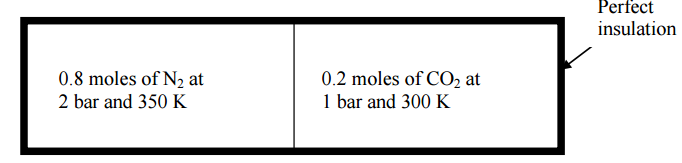
\includegraphics[width=0.7\columnwidth]{q20_thermo.png} \caption*{} \label{fig:q20_thermo} \end{figure}
    The membrane is ruptured and the gases are allowed to mix to form a homogeneous mixture at equilibrium. During this process there are no heat or work interactions between the tank contents and the surroundings. The final temperature at the equilibrium state in Kelvin is
    
    \hfill{\brak{\text{GATE XE 2014}}}
    \begin{enumerate}[label=\Alph*)]
        \begin{multicols}{4}
            \item 344.1
            \item 306.3
            \item 325.0
            \item 346.1
        \end{multicols}
    \end{enumerate}

    \item Two moist air streams MAS1 and MAS2 are mixed adiabatically. The details of MAS1 and MAS2 are given below in the table.
    \begin{table}[h!] \centering \caption*{} \label{tab:q21_thermo}
        \begin{tabular}{|l|c|c|} \hline
            & MAS1 & MAS2 \\ \hline
            h (kJ/kg of dry air) & 42 & 80 \\ \hline
            v (m$^3$/kg of dry air) & 0.85 & 0.9 \\ \hline
            Flow rate (m$^3$/min) & 85 & 90 \\ \hline
        \end{tabular}
    \end{table}
    With pressure remaining same and with no work interactions during the mixing process, the enthalpy of the mixed stream is \underline{\hspace{2cm}} kJ/kg of dry air.
    
    \hfill{\brak{\text{GATE XE 2014}}}
    \begin{enumerate}[label=\Alph*)]
        \begin{multicols}{4}
            \item 122
            \item 61
            \item 81
            \item 108
        \end{multicols}
    \end{enumerate}

    \item Consider the steady flow of air through an insulated nozzle. The pressure and temperature at the inlet are $120$ kPa and $320$ K, respectively. The outlet pressure is $1$ bar. The inlet velocity is very small and the air undergoes a reversible adiabatic process. The outlet velocity, in m/s, is
    
    \hfill{\brak{\text{GATE XE 2014}}}
    \begin{enumerate}[label=\Alph*)]
        \begin{multicols}{4}
            \item 303.7
            \item 180.7
            \item 5.7
            \item 127.3
        \end{multicols}
    \end{enumerate}
\end{enumerate}
\clearpage

\section*{F : POLYMER SCIENCE AND ENGINEERING}
\begin{enumerate}[label=\Alph*)]
    \item The estimation of the molecular weight of a polymer by gel permeation chromatography (GPC) is based on its
    
    \hfill{\brak{\text{GATE XE 2014}}}
    \begin{enumerate}
        \begin{multicols}{2}
            \item polarity
            \item size
            \item adsorption to stationary phase
            \item crystallinity
        \end{multicols}
    \end{enumerate}

    \item Elastomers are characterized by
    
    \hfill{\brak{\text{GATE XE 2014}}}
    \begin{enumerate}[label=\Alph*)]
        \item high modulus and high elongation at break
        \item high modulus and low elongation at break
        \item low modulus and high elongation at break
        \item low modulus and low elongation at break
    \end{enumerate}

    \item Thermodynamically, two polymers with enthalpy of mixing ($\Delta H$) and entropy of mixing ($\Delta S$) form a miscible blend at temperature T when
    
    \hfill{\brak{\text{GATE XE 2014}}}
    \begin{enumerate}[label=\Alph*)]
        \begin{multicols}{4}
            \item $\frac{\Delta H}{\Delta S} = 0.5T$
            \item $\frac{\Delta H}{\Delta S} = T$
            \item $\frac{\Delta H}{\Delta S} = 1.5T$
            \item $\frac{\Delta H}{\Delta S} = 2T$
        \end{multicols}
    \end{enumerate}

    \item The tensile strain of a uniformly extending plastic specimen of initial length $L_0$ and extended length $L$ is
    
    \hfill{\brak{\text{GATE XE 2014}}}
    \begin{enumerate}[label=\Alph*)]
        \begin{multicols}{4}
            \item $\frac{L_0}{L}$
            \item $\frac{L}{L_0}$
            \item $\frac{L_0}{L-L_0}$
            \item $\frac{L-L_0}{L_0}$
        \end{multicols}
    \end{enumerate}

    \item In natural rubber compounding, a peptizer is added
    
    \hfill{\brak{\text{GATE XE 2014}}}
    \begin{enumerate}[label=\Alph*)]
        \item at the beginning of the compounding cycle
        \item after the addition of filler
        \item at the end of the compounding cycle
        \item after the addition of antioxidant
    \end{enumerate}

    \item A continuous annular product is produced by
    
    \hfill{\brak{\text{GATE XE 2014}}}
    \begin{enumerate}[label=\Alph*)]
        \begin{multicols}{2}
            \item compression molding
            \item extrusion
            \item blow molding
            \item injection molding
        \end{multicols}
    \end{enumerate}

    \item Relate the three varieties of polyethylene in the left column with their chain structures given in the right column.
    \begin{table}[h!] \centering \caption*{} \label{tab:q7_polymer}
        \begin{tabular}{ll} \hline
            P. HDPE & 1. long as well as short branches \\
            Q. LDPE & 2. only short branches \\
            R. LLDPE & 3. no branches \\ \hline
        \end{tabular}
    \end{table}
    
    \hfill{\brak{\text{GATE XE 2014}}}
    \begin{enumerate}[label=\Alph*)]
        \begin{multicols}{4}
            \item P-1, Q-3, R-2
            \item P-3, Q-2, R-1
            \item P-2, Q-3, R-1
            \item P-3, Q-1, R-2
        \end{multicols}
    \end{enumerate}

    \item Match the following changes observed in the calorimetric analysis of a polymer sample when heat flow (y-axis) is plotted against temperature (x-axis):
    \begin{table}[h!] \centering \caption*{} \label{tab:q8_polymer}
        \begin{tabular}{ll} \hline
            P. step increase in heat flow & 1. crystallization \\
            Q. exothermic peak & 2. melting \\
            R. endothermic peak & 3. glass transition \\ \hline
        \end{tabular}
    \end{table}
    
    \hfill{\brak{\text{GATE XE 2014}}}
    \begin{enumerate}[label=\Alph*)]
        \begin{multicols}{4}
            \item P-1, Q-2, R-3
            \item P-2, Q-1, R-3
            \item P-3, Q-1, R-2
            \item P-3, Q-2, R-1
        \end{multicols}
    \end{enumerate}
    
    \item A Bingham plastic fluid is flowing under gravity, down a vertical plate, as a film. Find the appropriate match for the fully developed velocity profile of the fluid in the film, from among those shown below.
    
    \hfill{\brak{\text{GATE XE 2014}}}
    \begin{figure}[H]
        \centering \caption*{} \label{fig:q9_polymer_options}
        \begin{tabular}{cc}
        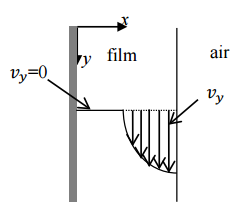
\includegraphics[width=0.3\columnwidth]{q9a_poly.png} & 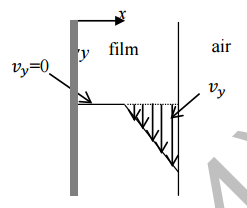
\includegraphics[width=0.3\columnwidth]{q9b_poly.png} \\
        (A) & (B) \\
        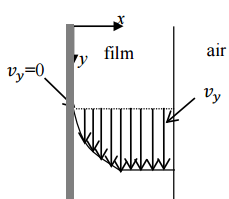
\includegraphics[width=0.3\columnwidth]{q9c_poly.png} & 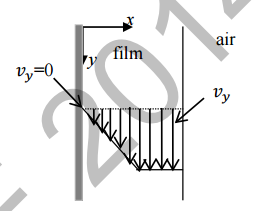
\includegraphics[width=0.3\columnwidth]{q9d_poly.png} \\
        (C) & (D)
        \end{tabular}
    \end{figure}
    
    \item Calculate the mass percent of the crystalline phase in a polymer sample of density $975$ kg/m$^3$. The density of amorphous phase is $866$ kg/m$^3$ and that of the crystalline phase is $996$ kg/m$^3$.
    
    \hfill{\brak{\text{GATE XE 2014}}}
    
    \item Find the rate of initiation (molL$^{-1}$s$^{-1}$) of a polymerization reaction using a peroxide initiator with a half life of $0.1$ s and efficiency of $70\%$, if the concentration of the initiator is $0.05$ molL$^{-1}$.
    
    \hfill{\brak{\text{GATE XE 2014}}}
    
    \item The constitutive equation of a shear thinning polymeric fluid is given by
    \begin{align*}
        \sigma = \frac{\mu_0 \dot{\gamma}}{1 + (\dot{\gamma}/\dot{\gamma}_0)}
    \end{align*}
    where $\sigma$ represents shear stress (Pa), and $\dot{\gamma}$, the corresponding shear rate (s$^{-1}$). The quantities $\mu_0 = 20$ Pas and $\dot{\gamma}_0 = 10$ s$^{-1}$ are constants. Find the apparent viscosity of the sample (Pas) when the applied shear rate is $40$ s$^{-1}$.
    
    \hfill{\brak{\text{GATE XE 2014}}}
    
    \item Identify the monomer for the polymer shown below prepared by ring opening metathesis polymerization.
    \begin{figure}[H] \centering 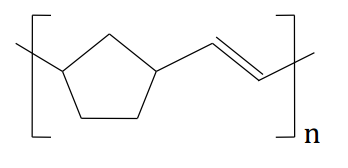
\includegraphics[width=0.4\columnwidth]{q13_poly.png} \caption*{} \label{fig:q13_poly} \end{figure}
    
    \hfill{\brak{\text{GATE XE 2014}}}
    \begin{figure}[H]
        \centering \caption*{} \label{fig:q13_poly_options}
        \begin{tabular}{cc}
        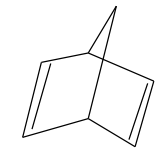
\includegraphics[width=0.3\columnwidth]{q13a_poly.png} & \includegraphics[width=0.3\columnwidth]{q13b_poly.png} \\
        (A) & (B) \\
        \includegraphics[width=0.3\columnwidth]{q13c_poly.png} & \includegraphics[width=0.3\columnwidth]{q13d_poly.png} \\
        (C) & (D)
        \end{tabular}
    \end{figure}
    
    \item The most appropriate order of toughness of nylon based materials is
    
    \hfill{\brak{\text{GATE XE 2014}}}
    \begin{enumerate}[label=\Alph*)]
        \item talc filled nylon < dry nylon < wet nylon
        \item dry nylon < wet nylon < talc filled nylon
        \item wet nylon < dry nylon < talc filled nylon
        \item wet nylon < talc filled nylon < dry nylon
    \end{enumerate}
    
    \item The shear rates involved in calendering ($\dot{\gamma}_{cal}$), compression molding ($\dot{\gamma}_{comp}$), extrusion ($\dot{\gamma}_{ext}$), and injection molding ($\dot{\gamma}_{inj}$) processes follow the order
    
    \hfill{\brak{\text{GATE XE 2014}}}
    \begin{enumerate}[label=\Alph*)]
        \begin{multicols}{2}
            \item $\dot{\gamma}_{inj} < \dot{\gamma}_{cal} < \dot{\gamma}_{ext} < \dot{\gamma}_{comp}$
            \item $\dot{\gamma}_{comp} < \dot{\gamma}_{ext} < \dot{\gamma}_{cal} < \dot{\gamma}_{inj}$
            \item $\dot{\gamma}_{comp} < \dot{\gamma}_{inj} < \dot{\gamma}_{ext} < \dot{\gamma}_{cal}$
            \item $\dot{\gamma}_{comp} < \dot{\gamma}_{cal} < \dot{\gamma}_{ext} < \dot{\gamma}_{inj}$
        \end{multicols}
    \end{enumerate}

    \item The dynamic mechanical response of a thermoplastic automotive component has shown a loss angle of $45\degree$ and storage modulus of $3500$ MPa. Calculate the loss modulus (MPa) of the component.
    
    \hfill{\brak{\text{GATE XE 2014}}}
    
    \item Match the terms in Column A with the appropriate terms in Column B:
    \begin{table}[h!] \centering \caption*{} \label{tab:q17_polymer}
        \begin{tabular}{ll} \hline
            \textbf{Column A} & \textbf{Column B} \\ \hline
            P. processability & 1. Rockwell scale \\
            Q. moisture permeation & 2. rubber modification \\
            R. hardness & 3. melt flow index \\
            S. fracture toughening & 4. Fick's law \\ \hline
        \end{tabular}
    \end{table}
    
    \hfill{\brak{\text{GATE XE 2014}}}
    \begin{enumerate}[label=\Alph*)]
        \begin{multicols}{2}
            \item P-3; Q-4; R-2; S-1
            \item P-3; Q-4; R-1; S-2
            \item P-4; Q-3; R-1; S-2
            \item P-4; Q-3; R-2; S-1
        \end{multicols}
    \end{enumerate}

    \item Match the following additives for plastics with their respective functions:
    \begin{table}[h!] \centering \caption*{} \label{tab:q18_polymer}
        \begin{tabular}{ll} \hline
            \textbf{Additive} & \textbf{Function} \\ \hline
            P. dilaurylthiodipropionate & 1. solid layer lubricant \\
            Q. graphite & 2. flame retardant \\
            R. antimony trioxide & 3. reinforcement \\
            S. carbon fibre & 4. antioxidant \\ \hline
        \end{tabular}
    \end{table}
    
    \hfill{\brak{\text{GATE XE 2014}}}
    \begin{enumerate}[label=\Alph*)]
        \begin{multicols}{2}
            \item P-4; Q-1; R-2; S-3
            \item P-1; Q-4; R-2; S-3
            \item P-4; Q-1; R-3; S-2
            \item P-1; Q-4; R-3; S-2
        \end{multicols}
    \end{enumerate}
    
    \item Match the following catalyst/initiator with the type of polymerization reaction:
    \begin{table}[h!] \centering \caption*{} \label{tab:q19_polymer}
        \begin{tabular}{ll} \hline
            \textbf{Catalyst/initiator} & \textbf{Polymerization reaction} \\ \hline
            P. butyl lithium & 1. Ziegler-Natta \\
            Q. TiCl$_4$ + Et$_3$Al & 2. cationic \\
            R. CuBr$_2$ & 3. anionic \\
            S. H$_2$SO$_4$ & 4. atom transfer radical polymerization \\ \hline
        \end{tabular}
    \end{table}
    
    \hfill{\brak{\text{GATE XE 2014}}}
    \begin{enumerate}[label=\Alph*)]
        \begin{multicols}{2}
            \item P-2; Q-1; R-4; S-3
            \item P-2; Q-4; R-1; S-3
            \item P-3; Q-1; R-4; S-2
            \item P-3; Q-4; R-1; S-2
        \end{multicols}
    \end{enumerate}
    
    \item For AIBN (mol. wt. = $164$ gmol$^{-1}$) initiated free radical polymerization of methyl methacrylate (mol. wt. = $100$ gmol$^{-1}$), where the termination is only by radical coupling, the $\bar{M}_n$ of PMMA is found to be $4636$ gmol$^{-1}$. Calculate the degree of polymerization.
    
    \hfill{\brak{\text{GATE XE 2014}}}
    
    \item A polymer solution is made by dissolving $5$ g of polymer in $1000$ ml of solvent. The flow time of the solvent and that of the polymer solution between two appropriate marks in a viscometer are $40$ s and $60$ s, respectively. The reduced viscosity (in dLg$^{-1}$) of the polymer solution is:
    
    \hfill{\brak{\text{GATE XE 2014}}}
    \begin{enumerate}[label=\Alph*)]
        \begin{multicols}{4}
            \item 0.25
            \item 0.50
            \item 1.0
            \item 1.5
        \end{multicols}
    \end{enumerate}
    
    \item The volume resistivity of a polymeric material is $10^7$ $\Omega$m. Find the resistance (in M$\Omega$) of a cube of the material of side $1$ cm. The direction of current flow is as shown in the figure below.
    \begin{figure}[H] \centering \includegraphics[width=0.2\columnwidth]{q22_poly.png} \caption*{} \label{fig:q22_poly} \end{figure}
    
    \hfill{\brak{\text{GATE XE 2014}}}
\end{enumerate}
\clearpage

\section*{G: FOOD TECHNOLOGY}
\begin{enumerate}
    \item The systematic name of sucrose is
    
    \hfill{\brak{\text{GATE XE 2014}}}
    \begin{enumerate}[label=\Alph*)]
        \item $\alpha$-D-Fructofuranosyl $(1 \rightarrow 2)$ $\beta$-D-Glucopyranoside
        \item $\alpha$-D-Glucopyranosyl $(1 \rightarrow 2)$ $\beta$-D-Fructofuranoside
        \item $\alpha$-D-Glucopyranosyl $(2 \rightarrow 1)$ $\beta$-D-Fructofuranoside
        \item $\alpha$-D-Fructofuranosyl $(2 \rightarrow 1)$ $\beta$-D-Glucopyranoside
    \end{enumerate}
    
    \item A non-hydrolyzable lipid is
    
    \hfill{\brak{\text{GATE XE 2014}}}
    \begin{enumerate}[label=\Alph*)]
        \begin{multicols}{4}
            \item Lecithin
            \item Arachidic acid
            \item Tocopherol
            \item Tristearin
        \end{multicols}
    \end{enumerate}
    
    \item The respiratory quotient (RQ) for the reaction $2\,\text{C}_{57}\text{H}_{110}\text{O}_6 + 163\,\text{O}_2 \rightarrow 114\,\text{CO}_2 + 110\,\text{H}_2\text{O}$ is
    
    \hfill{\brak{\text{GATE XE 2014}}}
    \begin{enumerate}[label=\Alph*)]
        \begin{multicols}{4}
            \item 0.70
            \item 1.14
            \item 1.43
            \item 0.14
        \end{multicols}
    \end{enumerate}
    
    \item Liver necrosis may be caused by the deficiency of
    
    \hfill{\brak{\text{GATE XE 2014}}}
    \begin{enumerate}[label=\Alph*)]
        \begin{multicols}{4}
            \item Vitamin A
            \item Vitamin D
            \item Vitamin K
            \item Vitamin E
        \end{multicols}
    \end{enumerate}
    
    \item Which of the following non-nutritive sweeteners contains similar calories per gram as that of sucrose?
    
    \hfill{\brak{\text{GATE XE 2014}}}
    \begin{enumerate}[label=\Alph*)]
        \begin{multicols}{4}
            \item Saccharin
            \item Aspartame
            \item Sucralose
            \item Cyclamate
        \end{multicols}
    \end{enumerate}
    
    \item The objective of heating milk to about $65^\circ$C before homogenization is to inactivate
    
    \hfill{\brak{\text{GATE XE 2014}}}
    \begin{enumerate}[label=\Alph*)]
        \begin{multicols}{4}
            \item Glucose oxidase
            \item Lipases
            \item Lactases
            \item Invertases
        \end{multicols}
    \end{enumerate}
    
    \item Make the correct match of the processes in Column I with the suitable materials/products in Column II
    \begin{table}[h!] \centering \caption*{} \label{tab:q7_food}
        \begin{tabular}{ll} \hline
            \textbf{Column I} & \textbf{Column II} \\ \hline
            1) Rendering & P) Lecithin \\
            2) Hydrogenation & Q) Fullers' earth \\
            3) Degumming & R) Lard \\
            4) Bleaching & S) Margarine \\ \hline
        \end{tabular}
    \end{table}
    
    \hfill{\brak{\text{GATE XE 2014}}}
    \begin{enumerate}[label=\Alph*)]
        \begin{multicols}{2}
            \item 1-R, 2-P, 3-Q, 4-S
            \item 1-P, 2-Q, 3-S, 4-R
            \item 1-R, 2-P, 3-S, 4-Q
            \item 1-R, 2-S, 3-P, 4-Q
        \end{multicols}
    \end{enumerate}

    \item A fruit juice of viscosity $\mu$ and density $\rho$ is agitated using an impeller of diameter D at a speed of N revolutions per minute. The terms $X = \frac{P}{\rho N^3 D^5}$, $Y = \frac{D^2 N \rho}{\mu}$, $Z = \frac{N^2 D}{g}$ represent three process related numbers, where P is power imparted by impeller and g is acceleration due to gravity. Which of the following is correct representation of these numbers?
    
    \hfill{\brak{\text{GATE XE 2014}}}
    \begin{enumerate}[label=\Alph*)]
        \begin{multicols}{2}
            \item X = Power, Y = Froude, Z = Reynolds
            \item X = Power, Y = Reynolds, Z = Froude
            \item X = Froude, Y = Reynolds, Z = Power
            \item X = Reynolds, Y = Power, Z = Froude
        \end{multicols}
    \end{enumerate}
    
    \item The energy required to reduce the size of a food material from a mean diameter of 12 mm to 4 mm is 10 kJ kg$^{-1}$. From Rittingers' law, the energy needed to reduce the same material from a diameter of 1.2 mm to 0.4 mm in kJ kg$^{-1}$ is \underline{\hspace{2cm}}.
    
    \hfill{\brak{\text{GATE XE 2014}}}
    
    \item Saccharomyces cerevisiae (mean doubling time 3.2 h) is grown in a batch fermenter with an operating volume of 12 m$^3$. A 2\% (v/v) inoculum, which contains 5 kg cells per 100 m$^3$ is mixed with the substrate. The residence time in the fermenter is 24 h and the density of broth is 1010 kg m$^{-3}$. The mass of S. cerevisiae obtained from the fermenter, in kg, is \underline{\hspace{2cm}}.
    
    \hfill{\brak{\text{GATE XE 2014}}}
    
    \item Make the correct combination of operations in Column I with the machines in Column II
    \begin{table}[h!] \centering \caption*{} \label{tab:q11_food}
        \begin{tabular}{ll} \hline
            \textbf{Column I} & \textbf{Column II} \\ \hline
            1) Rice milling & P) Pin mill \\
            2) Wheat milling & Q) Rubber rolls \\
            3) Mustard oil expelling & R) Break rolls \\
            4) Pepper grinding & S) Screw press \\ \hline
        \end{tabular}
    \end{table}
    
    \hfill{\brak{\text{GATE XE 2014}}}
    \begin{enumerate}[label=\Alph*)]
        \begin{multicols}{2}
            \item 1-Q, 2-R, 3-S, 4-P
            \item 1-R, 2-Q, 3-S, 4-P
            \item 1-Q, 2-P, 3-S, 4-R
            \item 1-Q, 2-R, 3-P, 4-S
        \end{multicols}
    \end{enumerate}

    \item The correct order for D$_{121}$ values of the spores of food spoilage bacteria in aqueous medium is
    
    \hfill{\brak{\text{GATE XE 2014}}}
    \begin{enumerate}[label=\Alph*)]
        \item B. stearothermophilus > C. sporogenes > C. botulinum type A > B. coagulans
        \item C. sporogenes > B. stearothermophilus > C. botulinum type A > B. coagulans
        \item C. botulinum type A > B. stearothermophilus > C. sporogenes > B. coagulans
        \item B. stearothermophilus > C. botulinum type A > C. sporogenes > B. coagulans
    \end{enumerate}
    
    \item Make the correct combination of pigments/microorganisms in Column I with the process/products in Column II
    \begin{table}[h!] \centering \caption*{} \label{tab:q13_food}
        \begin{tabular}{ll} \hline
            \textbf{Column I} & \textbf{Column II} \\ \hline
            1) Anthocyanin & P) Ropiness \\
            2) Chlorophyll & Q) Koji \\
            3) Bacillus subtilis & R) Glycosides \\
            4) Aspergillus oryzae & S) Porphyrins \\ \hline
        \end{tabular}
    \end{table}
    
    \hfill{\brak{\text{GATE XE 2014}}}
    \begin{enumerate}[label=\Alph*)]
        \begin{multicols}{2}
            \item 1-S, 2-R, 3-P, 4-Q
            \item 1-R, 2-S, 3-Q, 4-P
            \item 1-Q, 2-S, 3-P, 4-R
            \item 1-R, 2-S, 3-P, 4-Q
        \end{multicols}
    \end{enumerate}
    
    \item Make the correct combination of underlying principles in Column I with the processes in Column II
    \begin{table}[h!] \centering \caption*{} \label{tab:q14_food}
        \begin{tabular}{ll} \hline
            \textbf{Column I} & \textbf{Column II} \\ \hline
            1) Carbonyl derivatives react with free amino & P) Gelatinization \\
            \hspace{3mm} acids to yield aldehydes & \\
            2) Starch aggregates and forms micro-crystals & Q) Strecker degradation \\
            3) Starch granules swell and leach amylose & R) Caramelization \\
            4) Pyranose or furanose rings open up by & S) Retrogradation \\
            \hspace{3mm} pyrolytic reactions to form furfural & \\
            \hspace{3mm} derivatives & \\ \hline
        \end{tabular}
    \end{table}
    
    \hfill{\brak{\text{GATE XE 2014}}}
    \begin{enumerate}[label=\Alph*)]
        \begin{multicols}{2}
            \item 1-Q, 2-R, 3-P, 4-S
            \item 1-Q, 2-S, 3-P, 4-R
            \item 1-R, 2-S, 3-P, 4-Q
            \item 1-Q, 2-P, 3-S, 4-R
        \end{multicols}
    \end{enumerate}
    
    \item Which one of the following statements is FALSE?
    
    \hfill{\brak{\text{GATE XE 2014}}}
    \begin{enumerate}[label=\Alph*)]
        \item The peptide bond is planar offering restricted rotation around its axis.
        \item Full range of water activity is $0 \le a_w \le 1$ and it has well defined unit.
        \item The autooxidation of lipids proceeds via free radical mechanism.
        \item The carbonyl group of sugar reacts with nucleophilic amino group of amino acids in Amadori rearrangement.
    \end{enumerate}
    
    \item Which one of the following statements is TRUE?
    
    \hfill{\brak{\text{GATE XE 2014}}}
    \begin{enumerate}[label=\Alph*)]
        \item Pectate lyase hydrolyzes methyl ester bond of pectin.
        \item $\alpha$-Solanine is a non-toxic compound found in solanaceae plants.
        \item Egg proteins have lower digestibility than pea proteins.
        \item Lipoxygenase catalyses the conversion of cis, cis-1,4-pentadiene to hydroperoxides.
    \end{enumerate}
    
    \item Fish fillet having $84\%$ moisture (wet basis) is frozen from top using an air blast freezer maintained at $-32^\circ$C. The initial temperature of the fillet (density $1050$ kg m$^{-3}$) is $-2^\circ$C (freezing point). Convective heat transfer coefficient of air is $25$ Wm$^{-2}$K$^{-1}$, thermal conductivity of frozen fish is $1.0$ Wm$^{-1}$K$^{-1}$ and latent heat of crystallization is $340$ kJ kg$^{-1}$. The freezing time, in min, for a $20$ mm thick block of fish fillet weighing $1$ kg is \underline{\hspace{2cm}}.
    
    \hfill{\brak{\text{GATE XE 2014}}}
    
    \item Make the correct combination of properties in Column I with their dimensions in Column II
    \begin{table}[h!] \centering \caption*{} \label{tab:q18_food}
        \begin{tabular}{ll} \hline
            \textbf{Column I} & \textbf{Column II} \\ \hline
            1) Dynamic viscosity & P) m$^2$ s$^{-2}$ K$^{-1}$ \\
            2) Thermal conductivity & Q) kg m s$^{-2}$ \\
            3) Specific heat & R) kg m$^{-1}$ s$^{-1}$ \\
            4) Force & S) kg m s$^{-3}$ K$^{-1}$ \\ \hline
        \end{tabular}
    \end{table}
    
    \hfill{\brak{\text{GATE XE 2014}}}
    \begin{enumerate}[label=\Alph*)]
        \begin{multicols}{2}
            \item 1-R, 2-S, 3-Q, 4-P
            \item 1-Q, 2-S, 3-P, 4-R
            \item 1-R, 2-S, 3-P, 4-Q
            \item 1-S, 2-R, 3-P, 4-Q
        \end{multicols}
    \end{enumerate}
    
    \item The viscosity and density of a fruit juice at $21^\circ$C are $6.3 \times 10^{-3}$ Pa s and $1029$ kg m$^{-3}$, respectively. The juice flows at the rate of $0.12$ m$^3$ min$^{-1}$ in a $2.54$ cm inner diameter steel pipe. Correct combination of the Reynolds number ($N_{Re}$) and the nature of flow of juice is
    
    \hfill{\brak{\text{GATE XE 2014}}}
    \begin{enumerate}[label=\Alph*)]
        \begin{multicols}{2}
            \item $N_{Re} = 1048$, Laminar
            \item $N_{Re} = 2056$, Laminar
            \item $N_{Re} = 16375$, Turbulent
            \item $N_{Re} = 28656$, Turbulent
        \end{multicols}
    \end{enumerate}
    
    \item For a typical food sorption isotherm curve (Figure 1), which one of the following statements is CORRECT?
    \begin{figure}[H] \centering \includegraphics[width=0.6\columnwidth]{q20_food.png} \caption*{Figure 1: Food sorption isotherm curve} \label{fig:q20_food} \end{figure}
    
    \hfill{\brak{\text{GATE XE 2014}}}
    \begin{enumerate}[label=\Alph*)]
        \item Y-coordinate of A represents monolayer water content of food, A-B represents water absorbed in the multilayer within the food and B-C represents free water within the capillary network of the food.
        \item Y-coordinate of B represents monolayer water content of food, A-B represents water absorbed in the multilayer within the food and B-C represents free water within the capillary network of the food.
        \item Y-coordinate of A represents monolayer water content of food, Y-coordinate of B represents water absorbed in the multilayer within the food and B-C represents free water within the capillary network of the food.
        \item Y-coordinate of A represents monolayer water content of food, A-C represents water absorbed in the multilayer within the food and Y-coordinate of C represents free water within the capillary network of the food.
    \end{enumerate}
    
    \item $10,000$ kg milk (7\% fat) is passed through a cream separator to obtain cream (40\% fat) and skim milk (0.1\% fat). The cream, thus obtained, is churned to make butter of 80.5\% fat. If a loss of 0.5\% of initial milk fat occurs during the manufacturing process, the \% overrun is \underline{\hspace{2cm}}.
    
    \hfill{\brak{\text{GATE XE 2014}}}
    
    \item A $50$ mm thick pack of farm fresh berries is cooled at one side from $24^\circ$C to $7^\circ$C. The relevant properties of berries are: density $1025$ kg m$^{-3}$, specific heat $3.78$ kJ kg$^{-1}$K$^{-1}$, convective heat transfer coefficient $30$ Wm$^{-2}$K$^{-1}$, and thermal conductivity $0.3$ Wm$^{-1}$ K$^{-1}$. The Fourier number for a cooling span of $30$ min is \underline{\hspace{2cm}}.
    
    \hfill{\brak{\text{GATE XE 2014}}}
\end{enumerate}

\end{document}